% !TeX root = ../../Book1.tex
% 纲要标题：## 第7章　曲线的局部不变量与整体几何
% 纲要位置：几何学计划纲要.md，第 365 行。
% 正文状态：初稿；尚未正式审核。

% 纲要内容开始
% 
% > 本章目标与证明范围：以由微分不变量重建曲线为起点，再讨论闭合条件和整体曲率约束。Frenet 标架的适用范围、平行法标架和总曲率分别说明，避免把局部分类当成闭曲线分类。
% 
% 纲要内容结束

\chapter{曲线的局部不变量与整体几何}
\label{g1:ch:07}
\BookChapterNumber{g1:ch:07}

\begin{chapterabstract}
	曲线的弧长消除行走速度的影响，曲率与挠率记录单位长度内切向量和法方向的变化。本章先建立 Frenet 方程，说明零曲率点为何需要其他法标架，再完整证明由微分不变量重建曲线的存在与刚性唯一性。重建后的曲线是否闭合还需满足方向与位移的相合条件。对于闭曲线，切向映射把局部弯曲转成整体转角与总曲率，由此证明平面转角定理、凸性判据及空间曲线的 Fenchel 不等式，并说明结型所带来的进一步约束。
\end{chapterabstract}

\begin{learninggoals}
	\begin{itemize}
		\item 区分参数映射与轨迹，证明弧长公式与弧长重参数化，并正确处理方向和重复绕行。
		\item 推导曲率、挠率和 Frenet 方程，说明适用正则性及正曲率条件，构造能穿过零曲率点的平行法标架。
		\item 从连续系数线性方程的积分级数建立存在唯一性，利用正交性保持从给定不变量重建曲线。
		\item 分清保向刚性运动、空间反射和参数反向，检验周期数据何时真正给出闭曲线。
		\item 用切向角提升计算旋转次数，证明简单闭平面曲线的转角定理，并辨析曲率同号、凸性和简单性的关系。
		\item 将总曲率解释为球面切向曲线的长度，证明其下界与等号条件，读清非平凡结的总曲率限制所需的假设。
	\end{itemize}
\end{learninggoals}

把一根细线弯成圆，再弯成向上盘旋的螺线，我们可以在每一点描述它朝哪个方向走、向哪边弯。但这些描述还没有回答一个反问题：若只给出沿线的弯曲和扭转数据，是否足以重新摆出整根线？如果能够恢复，起点和朝向以外还会不会有别的自由？曲线基本定理将把这个问题化为一个标架方程和一次积分。

\ProseParagraphBreak

局部恢复以后，还需要问末端能否接回起点。圆柱螺线有恒定的曲率与挠率，却一直向上延伸；另一类平面曲线可以让切向量恰转一周，位置仍留下一个缺口。用 Frenet 方程重建正曲率曲线时，闭合还要求位置与 Frenet 标架在一周后相合。曲线真正闭合以后，其切向量还会受到额外限制：简单平面曲线的净转角只有一周，而空间闭曲线无论怎样扭动，总弯曲量至少为 \(2\pi\)。这些结论会把微分计算与整体几何接起来。

\ProseParagraphBreak

本章使用有限维微积分、内积与行列式。线性常微分方程的所需版本在正文证明；使用圆周的角度提升和 Jordan 分离定理时，将明确回引前两章的相应结果。参数化、曲率和经典平面曲线的进一步阅读可参见 Pressley 第二版的相应各节\cite[第1.1--1.4, 2.1--2.3, 3.1节]{Pressley2010}。关于非平凡结的严格总曲率下界，本章陈述结论并引用原始论文中的证明位置。

% !TeX root = ../../Book1.tex
% 纲要标题：### 7.1 参数、弧长与标架
% 纲要位置：几何学计划纲要.md，第 369 行。
% 正文状态：初稿；尚未正式审核。

% 纲要内容开始
% 
% * 正则参数化与重参数化
% * 弧长参数及方向选择
% * 曲率、挠率与 Frenet 方程
% * 零曲率点及替代法标架
% 
% 纲要内容结束

\section{参数、弧长与标架}
\label{g1:sec:0701}

同一条圆周可以匀速走过，也可以时快时慢地走过；速度和加速度会随走法改变，圆周的大小却没有改变。要从导数中提取形状信息，首先应消除这种速度选择。弧长参数使每单位参数恰好走过单位长度，随后切向量的变化才直接衡量曲线弯曲得多快。空间曲线还可能离开原来的弯曲平面，因此需要同时记录法方向怎样转动。

\subsection{正则参数化与重参数化}
\label{g1:subsec:0701:01}

本章主要讨论 \(\mathbb R^2\) 与 \(\mathbb R^3\) 中的曲线，使用标准 Euclid 内积；三维叉积按右手定向规定，即 \(\langle u\times v,w\rangle=\det(u,v,w)\)。当参数是一般的 \(t\) 时用上点表示求导；以弧长 \(s\) 为参数后，用撇号表示对 \(s\) 求导。这样做是为了在同一个公式中看清“每单位时间的变化”和“每单位长度的变化”。

\begin{definition}[正则曲线与重参数化]\label{g1:def:regular-curve}
	设 \(I,J\subset\mathbb R\) 是具有非空内部的区间，\(r\ge1\) 为整数。一个 \(C^r\) 映射 \(\alpha:I\to\mathbb R^n\) 称为 \(C^r\) 参数曲线；若 \(\dot\alpha(t)\ne0\) 对每个 \(t\in I\) 成立，就称其为\term[zhengzequxian]{正则曲线}[regular curve]。端点处的正则性按单侧导数理解，所说 \(C^r\) 均允许在端点附近作 \(C^r\) 延拓。若 \(h:J\to I\) 是导数处处非零的 \(C^r\) 双射，则 \(\beta=\alpha\circ h\) 称为 \(\alpha\) 的\term[chongcanshuhua]{重参数化}[reparametrization]；\(h'>0\) 时保方向，\(h'<0\) 时反方向。
\end{definition}

连续且不为零的 \(h'\) 在区间上符号恒定，所以这两种情况已经穷尽。逆函数连续可微，导数为 \(1/(h'\circ h^{-1})\)；对这个等式逐次求导便得到 \(C^r\) 正则性，因而定义中的 \(h\) 确实是微分同胚。链式法则给出 \(\dot\beta(u)=\dot\alpha(h(u))h'(u)\)，说明重参数化保持正则性。

\ProseParagraphBreak

正则性是参数映射的性质，不能只看轨迹集合。例如 \(t\mapsto(t^3,0)\) 的像是直线，导数却在 \(0\) 为零；它与 \(s\mapsto(s,0)\) 有相同轨迹，但 \(t\mapsto t^3\) 在 \(0\) 不满足这里的重参数化条件。另一方面，正则曲线可以自交：\(\alpha(t)=(\sin t,\sin2t)\) 的导数 \((\cos t,2\cos2t)\) 从不同时为零，而 \(\alpha(0)=\alpha(\pi)\)。速度不消失只保证局部能顺畅经过，不能保证不同时间不会经过同一点。

\begin{definition}[闭曲线与简单性]\label{g1:def:regular-closed-curve}
	设 \(P>0\)。一个 \(P\) 周期的 \(C^r\) 正则映射 \(\alpha:\mathbb R\to\mathbb R^n\) 称为 \(C^r\) 正则闭曲线，也视为定义在 \(\mathbb R/P\mathbb Z\) 上的映射。若 \(\alpha(t)=\alpha(u)\) 当且仅当 \(t-u\in P\mathbb Z\)，则称它为\term[jiandanbiquxian]{简单闭曲线}[simple closed curve]。不满足这个单射条件的闭曲线仍可能正则，甚至可能把一个简单轨迹重复走过多次。
\end{definition}

第六章中的 Jordan 曲线只要求圆周的连续嵌入；这里的简单正则闭曲线额外具有导数。若只给出 \([0,P]\) 上的公式，要求它成为 \(C^r\) 闭曲线，就必须检查端点处直到 \(r\) 阶的导数相合。仅有 \(\alpha(0)=\alpha(P)\) 还可能留下一个角点。

\subsection{弧长参数及方向选择}
\label{g1:subsec:0701:02}

内接折线的长度上确界给出曲线长度的几何定义。对连续曲线 \(\alpha:[a,b]\to\mathbb R^n\)，令
\[
	\ell(\alpha)=\sup_{a=t_0<\cdots<t_m=b}\sum_{i=1}^m\lVert\alpha(t_i)-\alpha(t_{i-1})\rVert.
\]
这个上确界可以为无穷；它把每次沿曲线走过的部分都计入，重复走圆周两次就会得到两倍周长。

\begin{proposition}[长度公式与弧长参数]\label{g1:prop:arc-length-param}
	设 \(\alpha:I\to\mathbb R^n\) 是 \(C^1\) 曲线。对每个紧子区间 \([a,b]\subset I\)，有
	\[
		\ell(\alpha|_{[a,b]})=\int_a^b\lVert\dot\alpha(t)\rVert\,\mathrm dt.
	\]
	若进一步 \(\alpha\) 为 \(C^r\) 正则曲线，\(r\ge1\)，固定 \(t_0\in I\)，定义
	\[
		s(t)=\int_{t_0}^t v(u)\,\mathrm du,\qquad v(t)=\lVert\dot\alpha(t)\rVert.
	\]
	则 \(s:I\to s(I)\) 是保方向的 \(C^r\) 微分同胚，\(\gamma(s)=\alpha(t(s))\) 满足 \(\lVert\gamma'(s)\rVert=1\)。它称为\term[huchangcanshu]{弧长参数}[arc-length parameter]下的曲线。两个描述同一条参数曲线的单位速率参数之间，只相差 \(s\mapsto s+c\) 或 \(s\mapsto -s+c\)。
\end{proposition}
\begin{proof}
	对任意分割，微积分基本定理及积分的三角不等式给出
	\[
		\sum_i\lVert\alpha(t_i)-\alpha(t_{i-1})\rVert
		=\sum_i\left\lVert\int_{t_{i-1}}^{t_i}\dot\alpha(t)\,\mathrm dt\right\rVert
		\le\int_a^b\lVert\dot\alpha(t)\rVert\,\mathrm dt.
	\]
	为了得到反向不等式，利用 \(\dot\alpha\) 在紧区间上的一致连续性。给定 \(\varepsilon>0\)，分割足够细时，在每个小区间内都有 \(\lVert\dot\alpha(t)-\dot\alpha(t_{i-1})\rVert<\varepsilon\)，于是
	\[
		\lVert\alpha(t_i)-\alpha(t_{i-1})\rVert
		\ge\lVert\dot\alpha(t_{i-1})\rVert(t_i-t_{i-1})-\varepsilon(t_i-t_{i-1}).
	\]
	求和并使分割网格趋于零，右侧的 Riemann 和趋于积分，再令 \(\varepsilon\to0\)，即得长度公式。

	正则时 \(v>0\)，所以 \(s'=v>0\)，\(s\) 严格递增。局部逆函数拼成整个像区间上的逆，且 \(\mathrm dt/\mathrm ds=1/v(t(s))\)。速度 \(v\) 属于 \(C^{r-1}\)，故 \(s\) 及其逆为 \(C^r\)，链式法则给出 \(\gamma'=\dot\alpha/v\)，其范数为 \(1\)。若另一单位速率表示是 \(\gamma(h(u))\)，则 \(1=\lVert\gamma'(h(u))h'(u)\rVert=|h'(u)|\)，连续性说明 \(h'\) 恒为 \(1\) 或恒为 \(-1\)，积分就得到结论。
\end{proof}

弧长反函数 \(t(s)\) 的存在由正速度保证。例如椭圆 \((a\cos t,b\sin t)\) 的弧长积分一般不容易显式反解。实际计算可以保留原来的参数，把每次弧长求导换成
\[
	\frac{\mathrm d}{\mathrm ds}=\frac1v\frac{\mathrm d}{\mathrm dt}.
\]
若曲线以 \(P\) 为周期，令 \(L=\int_0^P v(t)\,\mathrm dt\)，则 \(s(t+P)=s(t)+L\)，所以重参数化后成为 \(L\) 周期的单位速率闭曲线。这里改变的是行走速度，方向及走过的次数均保留。

\begin{example}[圆周与重复行走]\label{g1:exm:circle-speed}
	对半径 \(R>0\) 的圆 \(\alpha(t)=R(\cos t,\sin t)\)，有 \(v=R\)，以 \(\alpha(0)\) 为起点时 \(s=Rt\)，单位速率公式为 \(\gamma(s)=R(\cos(s/R),\sin(s/R))\)。一次周长是 \(2\pi R\)。若原参数在 \([0,4\pi]\) 上运行，总长度为 \(4\pi R\)；弧长化不会把两周自动变成一周。因此“形状相同”“参数等价”和“走过相同次数”是需要分别说明的事情。
\end{example}

\subsection{曲率、挠率与 Frenet 方程}
\label{g1:subsec:0701:03}

以下先用弧长。单位切向量 \(T=\gamma'\) 满足 \(\langle T,T\rangle=1\)，求导得到 \(\langle T',T\rangle=0\)：转向只能发生在法方向。单位长度内方向改变的大小，自然由 \(\lVert T'\rVert\) 衡量。

\begin{definition}[曲率与 Frenet 标架]\label{g1:def:frenet-frame}
	设 \(\gamma:I\to\mathbb R^3\) 为实区间 \(I\) 上的 \(C^2\) 单位速率曲线，令 \(T=\gamma'\)，定义其\term[qulv]{曲率}[curvature]为 \(\kappa(s)=\lVert T'(s)\rVert\)。在 \(\kappa>0\) 的部分，定义主法向量 \(N=T'/\kappa\) 与副法向量 \(B=T\times N\)。右手正交标架 \((T,N,B)\) 称为\term[Frenetbiaojia]{Frenet 标架}[Frenet frame]。\footnote{Frenet（Jean Frédéric Frenet，1816--1900）是法国数学家，以空间曲线的活动标架与相应微分公式著称。}若 \(\gamma\) 为 \(C^3\)，则 \(N,B\) 为 \(C^1\)，定义\term[naolv]{挠率}[torsion]为 \(\tau=-\langle B',N\rangle\)。
	\symidx{\(\kappa\)：空间曲线的非负曲率}
	\symidx{\(\tau\)：空间曲线的挠率}
\end{definition}

由 \(T,N\) 张成并经过曲线点的平面称为\term[mijiepingmian]{密切平面}[osculating plane]。Taylor 展开
\[
	\gamma(s+h)=\gamma(s)+hT(s)+\tfrac12h^2\kappa(s)N(s)+o(h^2)
\]
说明，在二阶近似中曲线沿着这张平面弯曲。副法向量 \(B\) 是这张平面的单位法向量，所以挠率衡量的是密切平面沿曲线的转动，正负号则依赖空间定向。

\begin{proposition}[Frenet 方程]\label{g1:prop:frenet-equations}
	设 \(\gamma:I\to\mathbb R^3\) 是 \(C^3\) 单位速率曲线，其曲率 \(\kappa\) 在整个实区间 \(I\) 上为正；以 \((T,N,B)\) 记其右手 Frenet 标架，以 \(\tau\) 记挠率。则
	\begin{equation}\label{g1:eq:frenet-equations}
		T'=\kappa N,\qquad N'=-\kappa T+\tau B,\qquad B'=-\tau N.
	\end{equation}
	这些等式也称为 Frenet--Serret 方程（Frenet--Serret equations）。\footnote{Serret（Joseph-Alfred Serret，1819--1885）是法国数学家，研究微分几何与分析；他独立给出了空间曲线的相应标架公式。}
\end{proposition}
\begin{proof}
	第一式就是 \(N\) 的定义。由 \(\langle B,B\rangle=1\) 得 \(B'\perp B\)；再对 \(\langle B,T\rangle=0\) 求导，有 \(\langle B',T\rangle=-\langle B,T'\rangle=-\kappa\langle B,N\rangle=0\)。因此 \(B'\) 只可能沿 \(N\)，其系数按定义是 \(-\tau\)。同样，\(N'\perp N\)，而
	\[
		\langle N',T\rangle=-\langle N,T'\rangle=-\kappa,\qquad
		\langle N',B\rangle=-\langle N,B'\rangle=\tau.
	\]
	把 \(N'\) 在正交基 \((T,N,B)\) 中展开就得到第二式。
\end{proof}

\begin{definition}[平面的有向曲率]\label{g1:def:signed-plane-curvature}
	在具有标准定向的平面 \(\mathbb R^2\) 中，令 \(J(x,y)=(-y,x)\)，即逆时针旋转 \(\pi/2\)。设 \(\gamma:I\to\mathbb R^2\) 为以弧长 \(s\) 为参数的 \(C^2\) 单位速率曲线，令 \(T=\gamma'\)。则 \((T,JT)\) 始终为正向正交标架；唯一的函数 \(k\) 使
	\[
		T'=k\,JT,\qquad k=\det(T,T')
	\]
	成立，称为\term[youxiangqulv]{有向曲率}[signed curvature]。曲线作为空间曲线时的非负曲率为 \(\kappa=|k|\)。左转时 \(k>0\)，右转时 \(k<0\)，该定义也允许 \(k=0\)。
	\symidx{\(k\)：定向平面曲线的有向曲率}
\end{definition}

在切向量落入一个小圆弧的区间内，可选连续角度 \(\theta\) 使 \(T=(\cos\theta,\sin\theta)\)。这时 \(T'=\theta'JT\)，所以 \(k=\theta'\)。角度换成 \(\theta+2m\pi\) 不改变导数；全局怎样选角度、闭合后角度能增加多少，将在\secref{g1:sec:0703}通过圆周覆盖来说明。

\begin{proposition}[一般参数下的计算公式]\label{g1:prop:curvature-torsion-formulas}
	设 \(\alpha:I\to\mathbb R^3\) 是 \(C^2\) 正则曲线，速度为 \(v=\lVert\dot\alpha\rVert\)。其非负曲率为
	\[
		\kappa=\frac{\lVert\dot\alpha\times\ddot\alpha\rVert}{v^3}.
	\]
	若 \(\alpha\) 为 \(C^3\) 且 \(\dot\alpha\times\ddot\alpha\ne0\)，则
	\[
		\tau=\frac{\det(\dot\alpha,\ddot\alpha,\dddot\alpha)}
		{\lVert\dot\alpha\times\ddot\alpha\rVert^2}.
	\]
	对 \(C^2\) 正则平面曲线，按参数递增的方向，其有向曲率为
	\[
		k=\frac{\det(\dot\alpha,\ddot\alpha)}{v^3}.
	\]
\end{proposition}
\begin{proof}
	写 \(T=\dot\alpha/v\)，则
	\[
		T'=\frac{\ddot\alpha}{v^2}-\frac{\dot v\,\dot\alpha}{v^3},\qquad
		\dot v=\frac{\langle\dot\alpha,\ddot\alpha\rangle}{v}.
	\]
	展开范数平方并使用 \(\lVert u\times w\rVert^2=\lVert u\rVert^2\lVert w\rVert^2-\langle u,w\rangle^2\)，就得曲率公式，这一计算在 \(\kappa=0\) 时也有效。平面的行列式计算同样消去平行于 \(\dot\alpha\) 的第二项，得到 \(k\) 的公式。

	在 \(\kappa>0\) 时，\(\dot\alpha=vT\)、\(\ddot\alpha=\dot vT+v^2\kappa N\)。对第二式按 \(t\) 求导，利用 Frenet 方程，\(\dddot\alpha\) 的 \(B\) 分量是 \(v^3\kappa\tau\)。因此
	\[
		\det(\dot\alpha,\ddot\alpha,\dddot\alpha)=v^6\kappa^2\tau,\qquad
		\lVert\dot\alpha\times\ddot\alpha\rVert^2=v^6\kappa^2,
	\]
	相除就得到挠率公式。分母不为零正是所需条件。
\end{proof}

\begin{example}[圆柱螺线]\label{g1:exm:circular-helix-invariants}
	设 \(a>0\)、\(b\in\mathbb R\)，考虑 \(\alpha(t)=(a\cos t,a\sin t,bt)\)。记 \(c=\sqrt{a^2+b^2}\)，则 \(v=c\)，并且
	\[
		\dot\alpha\times\ddot\alpha=(ab\sin t,-ab\cos t,a^2),\qquad
		\det(\dot\alpha,\ddot\alpha,\dddot\alpha)=a^2b.
	\]
	所以 \(\kappa=a/c^2\)、\(\tau=b/c^2\)。当 \(b=0\) 时是平面圆，挠率为零；当 \(b\ne0\) 时每转一周高度增加 \(2\pi b\)。曲率、挠率虽然都是常数，曲线却不闭合。下一节会反过来从给定的两个常数恢复这个模型。
\end{example}

反转行走方向和反转空间定向有不同影响。对 \(\widetilde\gamma(s)=\gamma(-s)\)，有 \(\widetilde T=-T\)、\(\widetilde N=N\)、\(\widetilde B=-B\)（右侧在 \(-s\) 处取值），由定义可得 \(\widetilde\kappa=\kappa\)、\(\widetilde\tau=\tau\)。平面的有向曲率却变成 \(\widetilde k=-k\)。若作空间等距变换 \(x\mapsto Qx+a\)，正交矩阵 \(Q\) 保持叉积的模，行列式则乘以 \(\det Q\)，故 \(\kappa\) 不变、\(\tau\) 乘以 \(\det Q\)；平面有向曲率也乘以平面变换的行列式。刚性变换具有上述形式，见\cref{g1:thm:isometry-affine}。

\subsection{零曲率点及替代法标架}
\label{g1:subsec:0701:04}

Frenet 标架在 \(\kappa=0\) 时不能用 \(N=T'/\kappa\) 定义。光滑曲线仍可经过这种点，也可具有连续的其他法向选择。例如 \(\alpha(t)=(t,t^3,0)\) 处处正则，而
\[
	k(t)=\frac{6t}{(1+9t^4)^{3/2}}.
\]
取 \(v=\sqrt{1+9t^4}\)，在 \(t\ne0\) 时，\(N=\operatorname{sgn}(t)(-3t^2,1,0)/v\)、\(B=\operatorname{sgn}(t)(0,0,1)\)，左右极限相反。给 \(N(0)\) 取任意值都不能使它连续。相反，平面法向 \(JT=(-3t^2,1,0)/v\) 在拐点处完全连续；让曲率带符号，就能避免将法向跟随弯曲侧翻转。

\ProseParagraphBreak

\cref{g1:fig:inflection-frame}对比了这两种法向选择：蓝色左法向连续变化，Frenet 主法向在左侧取相反方向。

% !TeX root = ../Book1.tex
\begin{figure}[htbp]
	\centering
	\begin{tikzpicture}[x=1.45cm,y=1.25cm,>=stealth,font=\small]
		\draw[->,gray] (-1.7,0)--(1.8,0) node[right]{\(x\)};
		\draw[->,gray] (0,-1.25)--(0,1.35) node[above]{\(y\)};
		\draw[thick,domain=-1.05:1.05,samples=80] plot(\x,{\x*\x*\x});
		\foreach \t in {-0.65,0,0.65}{
			\pgfmathsetmacro{\v}{sqrt(1+9*\t*\t*\t*\t)}
			\draw[blue!70!black,thick,->] (\t,{\t*\t*\t})--({\t-0.7*3*\t*\t/\v},{\t*\t*\t+0.7/\v});
		}
		\node[blue!70!black] at (-1.4,-0.1){\(JT\)};
		\draw[red!70!black,thick,dashed,->] (-0.65,-0.274625)--(-0.0998,-0.7087);
		\node[red!70!black] at (-0.12,-0.95){左侧的 \(N=-JT\)};
		\node[blue!70!black,align=left] at (2.8,0.8){右侧 \(N=JT\)\\但 \(JT\) 始终连续};
		\fill (0,0) circle(1.4pt);
	\end{tikzpicture}
	\caption[拐点两侧的法向选择]{曲线 \(y=x^3\) 的左法向 \(JT\) 连续穿过原点。Frenet 主法向指向弯曲的一侧，因而在左侧取 \(-JT\)、右侧取 \(JT\)，不能在原点连续拼接。}
	\label{g1:fig:inflection-frame}
\end{figure}


在三维中没有固定的平面旋转 \(J\) 可以选出唯一法向，但可以先在一个点选取一对正交法向，再规定它们沿曲线怎样继续。要求法向量的导数只沿切向，意味着法向量只作维持垂直所必需的转动，不额外在法平面内旋转。为构造这样的场，我们会使用\cref{g1:lem:linear-frame-ode}的连续系数线性常微分方程存在唯一性；该引理及其级数证明见下一节开头。

\begin{theorem}[平行法标架]\label{g1:thm:parallel-normal-frame}
	设 \(\gamma:I\to\mathbb R^3\) 为实区间 \(I\) 上的 \(C^2\) 单位速率曲线，令 \(T=\gamma'\)，固定 \(s_0\in I\) 和一组右手正交基 \((T(s_0),E_1^0,E_2^0)\)。存在唯一的 \(C^1\) 正交标架 \((T,E_1,E_2)\)，取给定初值并满足 \(E_i'\) 始终平行于 \(T\)。称它为\term[pingxingfabiaojia]{平行法标架}[parallel normal frame]。若 \(k_i=\langle T',E_i\rangle\)，则
	\begin{equation}\label{g1:eq:parallel-frame}
		T'=k_1E_1+k_2E_2,\qquad E_1'=-k_1T,\qquad E_2'=-k_2T,\qquad
		\kappa=\sqrt{k_1^2+k_2^2}.
	\end{equation}
	另一组同向平行法标架与这一组之间相差一个与 \(s\) 无关的法平面旋转。
\end{theorem}
\begin{proof}
	如果 \(E\perp T\) 且 \(E'\) 平行于 \(T\)，求导 \(\langle E,T\rangle=0\) 可得必须满足的方程
	\[
		E'=-\langle T',E\rangle T.
	\]
	它是未知向量 \(E\) 的线性方程，矩阵为 \(-T(T')^{\mathsf T}\)，系数连续。由上述线性方程引理，分别取初值 \(E_1^0,E_2^0\)，得到整个 \(I\) 上的唯一 \(C^1\) 解。还要确认解确实留在法平面中。直接计算
	\[
		\frac{\mathrm d}{\mathrm ds}\langle E_i,T\rangle
		=-\langle T',E_i\rangle\langle T,T\rangle+\langle E_i,T'\rangle=0.
	\]
	初值为零，所以始终垂直。继而 \((\langle E_i,E_j\rangle)'=0\)，因为 \(E_i',E_j'\) 都沿 \(T\)。因此长度与相互正交保持，标架的行列式连续且只能取 \(\pm1\)，初始右手性也保持。展开 \(T'\perp T\) 便得到全部方程及 \(\kappa\) 的表达式。

	若 \((\widetilde E_1,\widetilde E_2)\) 是另一组同向平行法标架，计算 \((\langle\widetilde E_i,E_j\rangle)'=0\)，两项都因法向与切向垂直而消失。所以变换矩阵常值，并且正交、行列式为 \(1\)，即一个固定的二维旋转。反过来，固定旋转后的标架仍满足同样的平行条件。
\end{proof}

平行法标架在 \(\kappa=0\) 时仍然有定义，此时 \(k_1=k_2=0\)，两个法向量的导数同时为零。在刚才的平面拐点例中，取 \(E_1=JT\)、\(E_2=(0,0,1)\)，便有 \(k_1=k\)、\(k_2=0\)。这两个带符号的分量可连续穿过零曲率点，使法向量保持连续。

\ProseParagraphBreak

在 \(\kappa>0\) 的区间，若写
\[
	N=\cos\theta\,E_1+\sin\theta\,E_2,\qquad
	B=-\sin\theta\,E_1+\cos\theta\,E_2,
\]
则 \(k_1=\kappa\cos\theta\)、\(k_2=\kappa\sin\theta\)。对第一式求导并代入\eqref{g1:eq:parallel-frame}，得到 \(N'=-\kappa T+\theta'B\)；与 Frenet 方程比较可知 \(\tau=\theta'\)。挠率因而是主法向相对于平行法标架的转角速度。在零曲率点，\((k_1,k_2)=(0,0)\) 没有确定的辐角，这正是不能一般地继续定义 Frenet 挠率的原因。

\ProseParagraphBreak

这里的存在唯一性是在一个参数区间上给定初值而言。若曲线闭合，沿一周继续平行法标架后，两个法向量未必回到起始值，可能相差一个固定旋转。初值唯一性确定沿途标架，一周后的法向旋转则记录闭合时的整体相合条件。

% !TeX root = ../../Book1.tex
% 纲要标题：### 7.2 曲线基本定理
% 纲要位置：几何学计划纲要.md，第 376 行。
% 正文状态：初稿；尚未正式审核。

% 纲要内容开始
% 
% * 标架常微分方程的存在与正交性保持
% * 从标架积分得到曲线
% * 刚性变换意义下的唯一性
% * 给定不变量与曲线闭合的额外条件
% 
% 纲要内容结束

\section{曲线基本定理}
\label{g1:sec:0702}

曲率与挠率是从曲线求导得到的两个函数。反过来，若只知道每一点弯曲多少、密切平面如何转动，能否恢复曲线？Frenet 方程提供了一种办法：先恢复三个随动的单位向量，再把切向量积分成位置。这里有两个需要分别回答的问题：方程是否有解，解出来的三个向量是否始终构成正交标架。Frenet 方程的斜对称系数将使内积导数为零，把初值处的正交性传到整个区间。

\subsection{标架常微分方程的存在与正交性保持}
\label{g1:subsec:0702:01}

下面以连续函数的积分、函数级数的一致收敛和微积分基本定理证明所需的线性常微分方程结论。以下区间均有非空内部；在区间包含的端点处，导数按单侧理解。

\begin{lemma}[连续系数线性方程]
	\label{g1:lem:linear-frame-ode}
	设 \(I\subseteq\mathbb R\) 是具有非空内部的区间，\(s_0\in I\)，\(A\colon I\rightarrow M_m(\mathbb R)\) 连续，端点处的导数按单侧理解。对任意 \(u_0\in\mathbb R^m\)，存在唯一的 \(C^1\) 函数 \(u\colon I\rightarrow\mathbb R^m\)，满足
	\[
		u'(s)=A(s)u(s),\qquad u(s_0)=u_0.
	\]
	特别地，连续矩阵系数方程 \(F'=FA\) 或 \(F'=AF\) 也有指定矩阵初值的唯一全区间解。
\end{lemma}

\begin{proof}
	把求导方程改写为积分方程
	\[
		u(s)=u_0+\int_{s_0}^s A(t)u(t)\,\mathrm{d}t.
	\]
	从常向量开始逐次积分，令
	\[
		u_0(s)=u_0,\qquad u_{j+1}(s)=\int_{s_0}^s A(t)u_j(t)\,\mathrm{d}t.
	\]
	这里 \(u_j\) 是将要相加的第 \(j\) 项，而不是第 \(j\) 次近似解。取包含 \(s_0\) 的任意紧子区间 \(J\subseteq I\)，令 \(M=\max_{t\in J}\lVert A(t)\rVert\)，范数取 Euclid 范数诱导的算子范数。反复积分并归纳可得
	\[
		\lVert u_j(s)\rVert\leq\lVert u_0\rVert\frac{M^j|s-s_0|^j}{j!},\qquad s\in J.
	\]
	当 \(s<s_0\) 时将积分反向后取绝对值，同一估计仍成立。于是级数 \(u=\sum_{j=0}^{\infty}u_j\) 在 \(J\) 上一致收敛。系数 \(A\) 有界，故可以把求和移入积分，得到上面的积分方程；被积函数连续，微积分基本定理便给出 \(u\in C^1\) 及 \(u'=Au\)。

	为证唯一性，设两解之差为 \(w\)，则 \(w(s_0)=0\) 且 \(w(s)=\int_{s_0}^s A(t)w(t)\,\mathrm{d}t\)。记 \(K=\max_J\lVert w\rVert\)，反复代入同一积分式，任意 \(j\geq0\) 均有
	\[
		\lVert w(s)\rVert\leq K\frac{M^j|s-s_0|^j}{j!}.
	\]
	右端随 \(j\to\infty\) 趋于零，故 \(w=0\)。

	每个 \(s\in I\) 都与 \(s_0\) 同处某个这样的紧区间。上述积分项在所有区间上由同一公式定义，因此得到 \(I\) 上的同一个解；无需假定 \(I\) 有界，也不要求 \(A\) 在整个 \(I\) 上有统一上界。矩阵方程 \(F'=AF\) 对每一列应用已证结论；\(F'=FA\) 则先转置，再对每一列应用它。
\end{proof}

上述阶乘估计解释了线性方程为何不会在有限的内部参数值处突然失去解：只要系数在这一点附近连续，紧区间上的整串积分仍然收敛。端点若不属于 \(I\)，则可能出现发散。例如 \(u'=u/(1-s)\) 在 \(I=(-\infty,1)\) 上的解可能在 \(s\to1\) 时发散。

\ProseParagraphBreak

把右手正交标架写成以向量为列的矩阵 \(F=(T,N,B)\)。由\cref{g1:prop:frenet-equations}，我们要解的是
\begin{equation}
	\label{g1:eq:frenet-matrix}
	F'=FA,\qquad
	A(s)=
	\begin{pmatrix}
		0&-\kappa(s)&0\\
		\kappa(s)&0&-\tau(s)\\
		0&\tau(s)&0
	\end{pmatrix}.
\end{equation}
第一列说 \(T'=\kappa N\)，第二列说 \(N'=-\kappa T+\tau B\)，第三列说 \(B'=-\tau N\)。矩阵 \(A\) 的各列记录导向量在当前标架中的系数，因此乘法写在右边。

\ProseParagraphBreak

行列式为 \(1\) 的正交矩阵组成\term[teshuzhengjiaoqun]{特殊正交群}[special orthogonal group]，这里记
\[
	\operatorname{SO}(3)\coloneqq\{Q\in M_3(\mathbb R):Q^{\mathsf T}Q=I,\ \det Q=1\}.
\]
它的列向量正好是右手正交标架。\symidx{\(\operatorname{SO}(3)\)：三维特殊正交群}

\begin{proposition}[斜对称系数保持标架]
	\label{g1:prop:skew-frame-orthogonality}
	设 \(I\subseteq\mathbb R\) 为具有非空内部的区间，\(s_0\in I\)，\(A\colon I\rightarrow M_3(\mathbb R)\) 连续且 \(A^{\mathsf T}=-A\)。设 \(F:I\to M_3(\mathbb R)\) 是方程 \(F'=FA\) 的 \(C^1\) 解，端点导数按单侧理解。若其初值 \(F(s_0)\) 属于 \(\operatorname{SO}(3)\)，则 \(F(s)\in \operatorname{SO}(3)\) 对每个 \(s\in I\) 成立。
\end{proposition}

\begin{proof}
	\cref{g1:lem:linear-frame-ode}给出全区间的 \(C^1\) 解。直接求导可得
	\[
		(FF^{\mathsf T})'=FAF^{\mathsf T}+FA^{\mathsf T}F^{\mathsf T}=0.
	\]
	因此 \(FF^{\mathsf T}=I\)。这使 \(F\) 可逆，且 \(F^{-1}=F^{\mathsf T}\)，从而也有 \(F^{\mathsf T}F=I\)。正交矩阵的行列式只能为 \(1\) 或 \(-1\)；它随 \(s\) 连续，而区间连通，所以只能恒等于初值 \(1\)。
\end{proof}

斜对称性恰好使长度与内积的变化抵消，因而把初值的一次正交条件传播到整个区间。

\subsection{从标架积分得到曲线}
\label{g1:subsec:0702:02}

现在可以把“弯曲和扭转决定形状”写成精确结论。条件 \(\kappa>0\) 保证 \(N=T'/\kappa\) 有意义；正则性条件则保证所得曲线确实具有本章用三阶导数定义的经典挠率。

\begin{theorem}[空间曲线基本定理：存在性]
	\label{g1:thm:space-curve-fundamental}
	设 \(I\subseteq\mathbb R\) 为具有非空内部的区间，\(\kappa\in C^1(I)\) 处处为正，\(\tau\in C^0(I)\)，端点处的导数按单侧理解。给定 \(s_0\in I\)、点 \(p_0\in\mathbb R^3\) 和右手正交标架 \((T_0,N_0,B_0)\)，存在唯一的 \(C^3\) 单位速率曲线 \(\gamma\colon I\rightarrow\mathbb R^3\)，使其曲率、挠率分别为 \(\kappa,\tau\)，并满足
	\[
		\gamma(s_0)=p_0,\qquad
		(T,N,B)(s_0)=(T_0,N_0,B_0).
	\]
	这一结论称为\term[quxianjibendingli]{曲线基本定理}[fundamental theorem of space curves]。
\end{theorem}

\begin{proof}
	用给定的 \(\kappa,\tau\) 组成\eqref{g1:eq:frenet-matrix}中的连续斜对称矩阵，解出初值 \(F(s_0)=(T_0,N_0,B_0)\) 的方程。由\cref{g1:prop:skew-frame-orthogonality}，三个列向量始终是右手正交单位向量。定义
	\begin{equation}
		\label{g1:eq:curve-frame-integral}
		\gamma(s)=p_0+\int_{s_0}^s T(t)\,\mathrm{d}t.
	\end{equation}
	于是 \(\gamma'=T\)，速率恒为 \(1\)。又因 \(T'=\kappa N\)，且 \(\kappa,N\) 都是 \(C^1\) 函数，故 \(T\in C^2\)，从而 \(\gamma\in C^3\)。这一步用到了 \(\kappa\in C^1\)，没有用到 \(\tau\) 可微。

	曲线的曲率为 \(\lVert\gamma''\rVert=\lVert\kappa N\rVert=\kappa\)。因 \(\kappa>0\)，其主法向量恰为构造中的 \(N\)，副法向量为 \(T\times N=B\)。最后 \(B'=-\tau N\)，所以其挠率 \(-\langle B',N\rangle\) 就是给定的 \(\tau\)。位置及标架的初值也由构造满足。

	任何满足条件的曲线，其 Frenet 标架都解同一矩阵初值问题，故由\cref{g1:lem:linear-frame-ode}与 \(F\) 相同。切向量既相同，位置初值也相同，积分式\eqref{g1:eq:curve-frame-integral}便使曲线相同。
\end{proof}

若只给连续的正函数 \(\kappa\) 和连续的 \(\tau\)，矩阵方程仍可解，积分仍给出 \(C^2\) 曲线，其 \(N,B\) 为 \(C^1\)。要得到 \(\gamma\in C^3\) 并使用涉及 \(\gamma'''\) 的经典挠率公式，还需加强数据的正则性。相反，若数据都光滑，反复对方程求导可知标架和曲线都光滑。

\begin{example}[常曲率和常挠率]
	\label{g1:exm:constant-curvature-helix}
	给定常数 \(\kappa_0>0\)、\(\tau_0\in\mathbb R\)，令 \(\omega=(\kappa_0^2+\tau_0^2)^{1/2}\)。曲线
	\[
		\gamma(s)=\left(
			\frac{\kappa_0}{\omega^2}\cos(\omega s),
			\frac{\kappa_0}{\omega^2}\sin(\omega s),
			\frac{\tau_0}{\omega}s
		\right)
	\]
	以单位速率运动，因为
	\[
		T=\left(-\frac{\kappa_0}{\omega}\sin(\omega s),
		\frac{\kappa_0}{\omega}\cos(\omega s),\frac{\tau_0}{\omega}\right).
	\]
	求导后得到 \(T'=\kappa_0N\)，其中
	\[
		N=(-\cos(\omega s),-\sin(\omega s),0),\qquad
		B=\left(\frac{\tau_0}{\omega}\sin(\omega s),
		-\frac{\tau_0}{\omega}\cos(\omega s),\frac{\kappa_0}{\omega}\right).
	\]
	直接计算 \(B'=-\tau_0N\)，所以曲率、挠率确为 \(\kappa_0,\tau_0\)。当 \(\tau_0=0\) 时得到半径 \(1/\kappa_0\) 的圆；当 \(\tau_0\ne0\) 时，第三坐标严格单调，得到不闭合的圆柱螺线。因而“曲率、挠率都是常数”并不蕴含闭合。
\end{example}

平面情形还能少解一个方程。由\cref{g1:def:signed-plane-curvature}，有向曲率 \(k\) 测量切向量向左转的速率。它可以为负，也可以经过零；只要改用转角，便不用除以曲率。

\begin{proposition}[由有向曲率重建平面曲线]
	\label{g1:prop:plane-curve-reconstruction}
	设 \(I\subseteq\mathbb R\) 为具有非空内部的区间，\(k\colon I\rightarrow\mathbb R\) 连续，端点处的导数按单侧理解。给定 \(s_0\in I\)、\(p_0\in\mathbb R^2\) 、\(\theta_0\in\mathbb R\) 及初始单位切向量 \((\cos\theta_0,\sin\theta_0)\)，令
	\[
		\theta(s)=\theta_0+\int_{s_0}^s k(t)\,\mathrm{d}t,\qquad
		\gamma(s)=p_0+\int_{s_0}^s(\cos\theta(t),\sin\theta(t))\,\mathrm{d}t.
	\]
	那么 \(\gamma\) 是具有这些初值和有向曲率 \(k\) 的唯一 \(C^2\) 单位速率平面曲线。
\end{proposition}

\begin{proof}
	定义式给出 \(\gamma'=T=(\cos\theta,\sin\theta)\)，而
	\[
		T'=k(-\sin\theta,\cos\theta)=kJT,\qquad J(x,y)=(-y,x).
	\]
	故 \(\det(T,T')=k\)，曲线为 \(C^2\) 且速率为 \(1\)。反之，任意具有有向曲率 \(k\) 的单位速率曲线都满足 \(\langle T,T'\rangle=0\) 以及 \(\det(T,T')=k\)，所以 \(T'=kJT\)。这是连续系数线性方程，指定初始切向量后由\cref{g1:lem:linear-frame-ode}唯一；再指定起点便唯一确定其积分。
\end{proof}

\subsection{刚性变换意义下的唯一性}
\label{g1:subsec:0702:03}

存在性定理指定了位置和整个标架，因而得到逐点相等的唯一性。通常说“不变量决定曲线”，并没有指定曲线在房间里的起点和朝向，此时应把平移与旋转造成的差别除去。\cref{g1:thm:isometry-affine}已经证明，Euclid 等距变换恰有形式 \(x\mapsto Qx+b\)，其中 \(Q\) 正交；保定向时还要求 \(\det Q=1\)。

\begin{proposition}[曲线的刚性唯一性]
	\label{g1:prop:curve-rigid-uniqueness}
	设 \(I\subseteq\mathbb R\) 为具有非空内部的区间，\(\gamma_1,\gamma_2\colon I\rightarrow\mathbb R^3\) 是其上的 \(C^3\) 单位速率曲线，曲率处处为正。若它们在同一参数 \(s\) 下有相同的曲率 \(\kappa(s)\) 和挠率 \(\tau(s)\)，则存在唯一的保定向 Euclid 等距变换 \(x\mapsto Qx+b\)，使
	\[
		\gamma_2(s)=Q\gamma_1(s)+b\qquad(s\in I).
	\]
	平面 \(C^2\) 单位速率曲线具有相同有向曲率时，也由唯一的保定向平面等距变换联系，不要求曲率非零。
\end{proposition}

\begin{proof}
	固定 \(s_0\in I\)，令两曲线的右手 Frenet 标架为 \(F_1,F_2\)，取
	\[
		Q=F_2(s_0)F_1(s_0)^{\mathsf T},\qquad
		b=\gamma_2(s_0)-Q\gamma_1(s_0).
	\]
	则 \(Q\in \operatorname{SO}(3)\)。因为数据相同，\(QF_1\) 和 \(F_2\) 满足同一方程 \(F'=FA\) 及同一初值，故相等。其第一列给出 \(\gamma_2'=Q\gamma_1'\)，积分即得所需等式。

	若另一个保定向刚性变换也逐参数匹配两曲线，对等式求一、二阶导数，得到它必须把 \(T_1(s_0)\)、\(N_1(s_0)\) 分别送到 \(T_2(s_0)\)、\(N_2(s_0)\)。保定向性又强制它把 \(B_1=T_1\times N_1\) 送到 \(B_2\)，因此正交部分必为 \(Q\)，平移部分再由起点确定。

	平面上，取唯一把初始单位切向量 \(T_1(s_0)\) 送到 \(T_2(s_0)\) 的旋转 \(Q\)，同样指定平移。旋转与 \(J\) 交换，故 \(QT_1\) 和 \(T_2\) 满足同一个方程 \(T'=kJT\) 及初值，于是曲线重合。唯一性只需初始切向量和起点。
\end{proof}

这里比较的是同一弧长参数下的函数。若先移动弧长原点，数据也要作相同平移；若逆转参数方向，也要先按\secref{g1:sec:0701}的变换规则重写数据。

\ProseParagraphBreak

还需分清参数反向与环境反射。若 \(\widetilde\gamma=Q\gamma+b\)，其中 \(Q\in O(3)\)，则 \(\widetilde T=QT\)、\(\widetilde N=QN\)，但
\[
	\widetilde B=\widetilde T\times\widetilde N=(\det Q)QB.
\]
这个叉积变换式可由 \(\langle u\times v,w\rangle=\det(u,v,w)\) 及正交矩阵的行列式直接验证。因此
\[
	\widetilde\kappa=\kappa,\qquad
	\widetilde\tau=-\langle\widetilde B',\widetilde N\rangle=(\det Q)\tau.
\]
环境反射把挠率变号；空间曲线的参数反向则不把挠率变号。若允许全部 Euclid 等距变换来比较曲线，相同曲率且挠率相反的一对曲线也可以互为镜像，挠率的整体改号对应镜像。

\subsection{给定不变量与曲线闭合的额外条件}
\label{g1:subsec:0702:04}

闭合要求走过一周的总位移为零，并要求参数接点处的切向量与法向量相容。标架方程的初值唯一性可以把这两项条件写成一周后的数据。

\begin{proposition}[周期数据的闭合判据]
	\label{g1:prop:periodic-curve-closure}
	设 \(L>0\)，\(\kappa\in C^1(\mathbb R)\) 为处处正的 \(L\) 周期函数，\(\tau\in C^0(\mathbb R)\) 也为 \(L\) 周期函数。令 \(A=\begin{psmallmatrix}0&-\kappa&0\\\kappa&0&-\tau\\0&\tau&0\end{psmallmatrix}\)，取任意 \(F(0)\in\operatorname{SO}(3)\)，以 \(F:\mathbb R\to M_3(\mathbb R)\) 解 \(F'=FA\)，即\eqref{g1:eq:frenet-matrix}。以 \(T\) 记 \(F\) 的第一列，给定 \(p_0\in\mathbb R^3\)，并令 \(\gamma(s)=p_0+\int_0^sT(t)\,\mathrm{d}t\)。则 \(\gamma\) 为 \(L\) 周期曲线，当且仅当
	\begin{equation}
		\label{g1:eq:space-closure-conditions}
		F(L)=F(0),\qquad \int_0^L T(s)\,\mathrm{d}s=0.
	\end{equation}
	此时它给出 \(\mathbb R/L\mathbb Z\) 上的 \(C^3\) 正则参数曲线，但不一定单射。条件是否成立与初始位置和右手标架的选择无关。
\end{proposition}

\begin{proof}
	若 \(\gamma\) 为 \(L\) 周期，则 \(\gamma'\)、\(\gamma''\) 也为 \(L\) 周期。由 \(T=\gamma'\)、\(N=\gamma''/\kappa\) 以及 \(B=T\times N\)，可知 \(F(L)=F(0)\)；积分条件就是 \(\gamma(L)-\gamma(0)=0\)。

	反过来，由系数的周期性，函数 \(F(s+L)\) 和 \(F(s)\) 解同一矩阵方程。它们在 \(s=0\) 的值相同，唯一性便给出 \(F(s+L)=F(s)\) 对所有 \(s\) 成立。特别地 \(T\) 周期，故函数 \(\int_s^{s+L}T(t)\,\mathrm{d}t\) 的导数为 \(T(s+L)-T(s)=0\)，它恒等于 \(\int_0^L T(t)\,\mathrm{d}t=0\)。于是 \(\gamma(s+L)=\gamma(s)\)。

	周期的 \(C^3\) 函数可通过商映射 \(\mathbb R\to\mathbb R/L\mathbb Z\) 下降：在每个长度小于 \(L\) 的坐标弧内用原函数表示，重叠处只差整数倍 \(L\) 的参数平移，因而各阶导数相容；速率仍为 \(1\)。改变初始位置只平移曲线，改变右手标架则使所有 \(F,T\) 同时左乘一个固定的 \(Q\in \operatorname{SO}(3)\)。这些操作都不改变\eqref{g1:eq:space-closure-conditions}中的两个等式是否成立。
\end{proof}

为看清周期性实际给出的内容，令 \(Q=F(L)F(0)^{\mathsf T}\)。即使 \(Q\ne I\)，方程唯一性仍然给出 \(F(s+L)=QF(s)\)。进一步积分得到
\[
	\gamma(s+L)=Q\gamma(s)+\bigl(\gamma(L)-Q\gamma(0)\bigr).
\]
所以周期数据保证，相邻两段长度 \(L\) 的曲线之间都相差同一个刚性运动；只有满足闭合条件时，这种重复才成为逐参数的闭合。

\ProseParagraphBreak

平面上，若 \(k\) 是连续的 \(L\) 周期函数，则\cref{g1:prop:plane-curve-reconstruction}把闭合条件化为
\begin{equation}
	\label{g1:eq:plane-closure-conditions}
	\int_0^L k(s)\,\mathrm{d}s\in2\pi\mathbb Z,\qquad
	\int_0^L \cos\theta(s)\,\mathrm{d}s=0,\qquad
	\int_0^L \sin\theta(s)\,\mathrm{d}s=0.
\end{equation}
第一个条件是切向量回到初始方向，后两个条件是位置回到起点。其充分性来自 \(T(s+L)=T(s)\) 与位移为零；必要性则由闭曲线的切向量周期和积分式得到。总转角为整周不能代替位移条件。

\begin{example}[转满一周却没有闭合]
	\label{g1:exm:turning-with-displacement}
	取 \(0<\varepsilon<1\)，先以转角 \(\theta\) 为参数，定义
	\[
		r(\theta)=\left(
			\sin\theta+\varepsilon\left(\frac{\theta}{2}+\frac{\sin2\theta}{4}\right),
			1-\cos\theta+\frac{\varepsilon}{2}\sin^2\theta
		\right).
	\]
	其导数为
	\[
		r'(\theta)=(1+\varepsilon\cos\theta)(\cos\theta,\sin\theta),
	\]
	速率严格为正。弧长为 \(s=\theta+\varepsilon\sin\theta\)，这是严格递增且映满 \(\mathbb R\) 的光滑函数；令其反函数为 \(\theta(s)\)。于是 \(\gamma(s)=r(\theta(s))\) 是单位速率曲线，有向曲率
	\[
		k(s)=\frac{1}{1+\varepsilon\cos\theta(s)}>0.
	\]
	由 \(s(\theta+2\pi)=s(\theta)+2\pi\)，得 \(\theta(s+2\pi)=\theta(s)+2\pi\)，故 \(k\) 以 \(L=2\pi\) 为周期，切向量也恰转一周。但是
	\[
		\gamma(2\pi)-\gamma(0)=r(2\pi)-r(0)=(\pi\varepsilon,0)\ne0.
	\]
	因此它满足标架接合条件却不满足位移条件。把它放入 \(\mathbb R^3\) 的水平面，便同时得到 \(\kappa=k>0,\tau=0\) 的空间反例。
\end{example}

\begin{figure}[htbp]
	\centering
	% !TeX root = ../Book1.tex
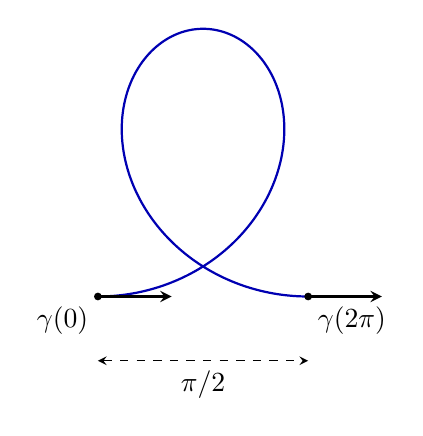
\begin{tikzpicture}[x=1.7cm,y=1.7cm,>=stealth]
	\draw[blue!70!black,thick,domain=0:360,samples=161,smooth,variable=\t] plot ({sin(\t)+0.5*(\t*pi/360+sin(2*\t)/4)},{1-cos(\t)+0.25*sin(\t)^2});
	\fill (0,0) circle (1.4pt) node[below left] {\(\gamma(0)\)};
	\fill ({pi/2},0) circle (1.4pt) node[below right] {\(\gamma(2\pi)\)};
	\draw[->,thick] (0,0)--(0.55,0);
	\draw[->,thick] ({pi/2},0)--({pi/2+0.55},0);
	\draw[<->,dashed] (0,-0.48)--node[below] {\(\pi/2\)} ({pi/2},-0.48);
\end{tikzpicture}

	\caption[切向量接合与位置闭合]{切向量接合与位置闭合。\(\varepsilon=\tfrac12\) 时，曲线转角从 \(0\) 增至 \(2\pi\)，两端的切向量相同，但端点相差 \((\pi/2,0)\)。箭头只表示相应端点的切向方向。}
	\label{g1:fig:closure-displacement}
\end{figure}

正面的例子是 \(k(s)=1/R\)、\(L=2\pi R\)，取初始切向量为 \((1,0)\)，积分得到
\[
	\gamma(s)=\bigl(R\sin(s/R),R(1-\cos(s/R))\bigr).
\]
三项闭合条件都成立，曲线恰为圆。若改用周期 \(4\pi R\)，同一公式仍满足条件，却把圆走了两遍。简单性还要求一个周期内只经过每个点一次。

% !TeX root = ../../Book1.tex
% 纲要标题：### 7.3 平面闭曲线的绕转
% 纲要位置：几何学计划纲要.md，第 383 行。
% 正文状态：初稿；尚未正式审核。

% 纲要内容开始
% 
% * 切向映射的次数
% * 转角定理与简单闭曲线
% * 曲率符号、凸性及反例
% 
% 纲要内容结束

\section{平面闭曲线的绕转}
\label{g1:sec:0703}

沿一条平面闭曲线走一周，位置回到原点，切向量也回到原方向；但连续记录的切向角可能多转了几周。这个整周差把局部的有向曲率同闭曲线的整体形状联系起来。简单性将这个整数限制为 \(1\) 或 \(-1\)，曲率同号则使切向角单调，从而把转角与凸性联系起来。

\subsection{切向映射的次数}
\label{g1:subsec:0703:01}

设 \(\gamma:\mathbb R/L\mathbb Z\rightarrow\mathbb R^2\) 是 \(C^1\) 正则闭曲线；用弧长参数时，\(L\) 是总长，\(T(s)=\gamma'(s)\in S^1\)。闭合在这里包含参数接点的导数相容，因而 \(T(0)=T(L)\)。\cref{g1:lem:circle-angle-lift}说明，给定初始角度后，可以沿区间 \([0,L]\) 唯一地选择连续函数 \(\theta\)，使
\[
	T(s)=(\cos\theta(s),\sin\theta(s)).
\]
前章把圆周角度按整周归一为 \(e^{2\pi iu}\)；本节使用弧度，所以这里的 \(\theta\) 是那里角度提升的 \(2\pi\) 倍。等式 \(T(0)=T(L)\) 只保证 \(\theta(L)-\theta(0)\in2\pi\mathbb Z\)，不要求这个差为零。

\begin{definition}[旋转次数]\label{g1:def:rotation-index}
	设 \(P>0\)，\(\gamma:\mathbb R/P\mathbb Z\to\mathbb R^2\) 为 \(C^1\) 正则闭曲线，令 \(T(t)=\gamma'(t)/\|\gamma'(t)\|\)，并取 \(T\) 在 \([0,P]\) 上的连续角度提升 \(\theta\)。单位切向映射的\term[cishu]{次数}[degree]称为曲线的\term[xuanzhuancishu]{旋转次数}[rotation index]，记为
	\[
		\operatorname{rot}(\gamma)\coloneqq\deg T
		=\frac{\theta(P)-\theta(0)}{2\pi}\in\mathbb Z.
	\]
	若采用弧长参数，则以总长 \(L\) 替代 \(P\)。这里次数就是\cref{g1:thm:circle-fundamental}中圆周映射沿定义域正向一周的绕数；任意两个角度提升相差常数 \(2\pi m\)，故右边不依赖初始角度的选择。
\end{definition}

切向映射在方向圆周上走，原曲线在位置平面上走。旋转次数记录前者，不能与原曲线绕某个指定点的绕数混同：后者需要先选一个不在曲线上的点，而前者不需要这样一个点。

\begin{proposition}[有向曲率的整周积分]\label{g1:prop:total-turning}
	设 \(\gamma:\mathbb R/L\mathbb Z\rightarrow\mathbb R^2\) 是 \(C^2\) 弧长参数正则闭曲线，\(k\) 是按 \(T'=kJT\) 定义的有向曲率，其中 \(J(x,y)=(-y,x)\)。则其连续切向角提升是 \(C^1\) 的，且
	\begin{equation}\label{g1:eq:total-signed-curvature}
		k(s)=\theta'(s),\qquad \int_0^L k(s)\,\mathrm{d}s=2\pi\operatorname{rot}(\gamma).
	\end{equation}
	对一般正则参数 \(t\in[0,P]\)，同一公式写为
	\[
		2\pi\operatorname{rot}(\gamma)
		=\int_0^P\frac{\det(\dot\gamma(t),\ddot\gamma(t))}{|\dot\gamma(t)|^2}\,\mathrm{d}t.
	\]
\end{proposition}
\begin{proof}
	在任一小开弧上，圆周有光滑角度坐标。连续提升在这样的坐标区间内与该局部角度相差固定的 \(2\pi\) 整数倍，所以它具有与 \(T\) 相同的 \(C^1\) 正则性。微分给出
	\[
		T'(s)=\theta'(s)(-\sin\theta(s),\cos\theta(s))=\theta'(s)JT(s).
	\]
	与有向曲率的定义比较得到 \(k=\theta'\)，然后应用微积分基本定理。一般参数下，\cref{g1:prop:arc-length-param}给出 \(\mathrm{d}s=|\dot\gamma|\,\mathrm{d}t\)，而有向曲率公式为 \(k=\det(\dot\gamma,\ddot\gamma)/|\dot\gamma|^3\)；将这两个等式相乘即得最后一式。
\end{proof}

\begin{proposition}[方向与连续变形]\label{g1:prop:rotation-invariance}
	旋转次数在保向正则重参数化和保向平面刚体运动下不变；反向重参数化或平面反射各使它变号。若 \(\gamma_u:\mathbb R/P\mathbb Z\rightarrow\mathbb R^2\) 是一族闭曲线，\((t,u)\mapsto\gamma_u(t)\) 与 \((t,u)\mapsto\partial_t\gamma_u(t)\) 均连续，且后者处处非零，\(u\in[0,1]\)，则 \(\operatorname{rot}(\gamma_u)\) 与 \(u\) 无关。
\end{proposition}
\begin{proof}
	保向重参数化只按原次序走过切向映射；反向重参数化使切向量成为原切向量的负向并逆序走过。取负向只给切向角加上 \(\pi\)，逆序则把总增量变号。保向平面刚体运动给角度加一个常数，反射把角度变为某个常数减去原角度，这证明前两句。

	对连续变形，单位切向量
	\[
		T_u(t)=\frac{\partial_t\gamma_u(t)}{|\partial_t\gamma_u(t)|}
	\]
	构成圆周映射的连续同伦。把平面识别为复平面，考虑 \(T_u(t)/T_u(0)\)，就得到基点始终为 \(1\) 的环路同伦。\cref{g1:thm:circle-fundamental}的同伦不变性使它们的绕数相同，而除以 \(T_u(0)\) 只减去常数角度。
\end{proof}

命题最后一类变形称为\term[zhengzetonglun]{正则同伦}[regular homotopy]：在变形中允许曲线穿过自身，但切向量不能消失。旋转次数因而是正则同伦的不变量。

\subsection{转角定理与简单闭曲线}
\label{g1:subsec:0703:02}

简单闭曲线要求 \(\gamma:\mathbb R/L\mathbb Z\rightarrow\mathbb R^2\) 单射。\cref{g1:thm:jordan-separation}给出其有界内部 \(\Omega\) 和无界外部。在曲线每一点，以切线为横轴，正则性使一小段曲线成为 \(C^1\) 函数的图像；把坐标矩形取得足够小，还能避开其余曲线。图像分出的两侧恰分别属于内部和外部，因为两者的边界都是整条曲线。内部处于行进方向的左侧还是右侧，是随参数局部不变的选择，故在整个参数圆周上一致。称内部位于左侧的行进方向为正向；反转参数即可在两种方向间转换。

\begin{theorem}[转角定理]\label{g1:thm:turning-tangent}
	设 \(\gamma:\mathbb R/L\mathbb Z\rightarrow\mathbb R^2\) 是 \(C^1\) 正则简单闭曲线。正向参数下 \(\operatorname{rot}(\gamma)=1\)，反向参数下 \(\operatorname{rot}(\gamma)=-1\)。特别地，若 \(\gamma\) 为 \(C^2\) 弧长参数曲线，则
	\[
		\int_0^L k(s)\,\mathrm{d}s=
		\begin{cases}
			2\pi,&\text{正向},\\
			-2\pi,&\text{反向}.
		\end{cases}
	\]
\end{theorem}

简单曲线可以有许多凹陷，切向角也可以来回变化。用两个点合拢时的弦方向表示相切方向，就能在参数三角形上统一记录这些变化。\cref{g1:fig:chord-triangle}显示了三条边各自承担的角度变化。

\begin{figure}[htbp]
	\centering
	% !TeX root = ../Book1.tex
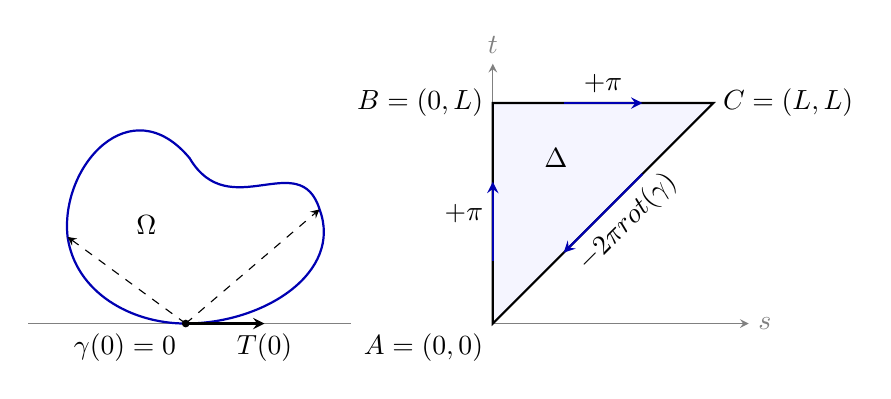
\begin{tikzpicture}[x=1cm,y=1cm,>=stealth]
	\begin{scope}[shift={(1.7,0.25)}]
		\draw[gray] (-2,0)--(2.1,0);
		\draw[thick,blue!70!black] (0,0) .. controls (1,0) and (2,0.65) .. (1.7,1.45) .. controls (1.45,2.25) and (0.55,1.25) .. (0.05,2.1) .. controls (-0.7,3) and (-1.6,2) .. (-1.5,1.1) .. controls (-1.4,0.4) and (-0.7,0) .. (0,0);
		\draw[->,thick] (0,0)--(1,0) node[below] {\(T(0)\)};
		\draw[dashed,->] (0,0)--(1.7,1.45);
		\draw[dashed,->] (0,0)--(-1.5,1.1);
		\fill (0,0) circle (1.4pt);
		\node[below left] at (0,0) {\(\gamma(0)=0\)};
		\node at (-0.5,1.25) {\(\Omega\)};
	\end{scope}
	\begin{scope}[shift={(5.6,0.25)}]
		\fill[blue!4] (0,0)--(0,2.8)--(2.8,2.8)--cycle;
		\draw[->,gray] (0,0)--(3.25,0) node[right] {\(s\)};
		\draw[->,gray] (0,0)--(0,3.3) node[above] {\(t\)};
		\draw[thick] (0,0)--(0,2.8)--(2.8,2.8)--cycle;
		\draw[->,blue!70!black,thick] (0,0.8)--(0,1.8);
		\draw[->,blue!70!black,thick] (0.9,2.8)--(1.9,2.8);
		\draw[->,blue!70!black,thick] (1.9,1.9)--(0.9,0.9);
		\node[left] at (0,1.4) {\(+\pi\)};
		\node[above] at (1.4,2.8) {\(+\pi\)};
		\node[rotate=45,below] at (1.5,1.5) {\(-2\pi\operatorname{rot}(\gamma)\)};
		\node at (0.8,2.1) {\(\Delta\)};
		\node[below left] at (0,0) {\(A=(0,0)\)};
		\node[left] at (0,2.8) {\(B=(0,L)\)};
		\node[right] at (2.8,2.8) {\(C=(L,L)\)};
	\end{scope}
\end{tikzpicture}

	\caption[弦方向的参数三角形]{左图以曲线最低点为基点，此点发出的所有弦均指向闭上半平面。右图的两条直角边分别记录基点弦方向及其负向，各有角增量 \(\pi\)；斜边逆向记录切向映射。图中曲线仅为示意，证明不要求凸性。}
	\label{g1:fig:chord-triangle}
\end{figure}

\begin{proof}
	先取弧长参数；\(C^1\) 正则性足以使用\cref{g1:prop:arc-length-param}，旋转次数不因这种保向重参数化而改变。旋转、平移平面并移动参数起点，使 \(\gamma(0)=\gamma(L)=0\) 是曲线第二坐标的最小点，整条曲线位于 \(y\geq0\)。该点的切向量水平。正向时 \(T(0)=(1,0)\)：最低点下方属于无界外部，局部内部在切线的上侧，正向要求它位于左方。

	在闭三角形
	\[
		\Delta=\{(s,t):0\leq s\leq t\leq L\}
	\]
	上定义一个圆周值映射。对 \(s<t\)、\((s,t)\ne(0,L)\)，令
	\[
		F(s,t)=\frac{\gamma(t)-\gamma(s)}{|\gamma(t)-\gamma(s)|}.
	\]
	简单性保证分母不为零。在对角线上令 \(F(s,s)=T(s)\)，在余下角点令 \(F(0,L)=-T(0)\)。这些赋值确实连续。对角线附近，
	\[
		\frac{\gamma(t)-\gamma(s)}{t-s}
		=\frac1{t-s}\int_s^t T(v)\,\mathrm{d}v
	\]
	一致趋近相应的单位切向量；这是紧区间上 \(T\) 一致连续的直接结果。在角点 \((0,L)\) 附近，设 \(a=s\)、\(b=L-t\)，由两端相容的导数 \(T(0)=T(L)\)，
	\[
		\gamma(L-b)-\gamma(a)=-(a+b)T(0)+o(a+b).
	\]
	归一化后恰趋向 \(-T(0)\)，也包括 \(a=0\) 或 \(b=0\) 的情形。

	令 \(A=(0,0)\)、\(B=(0,L)\)、\(C=(L,L)\)。沿 \(A\to B\) 走，\(F(0,t)\) 是从原点发出的弦方向，始终在闭上半圆。因此其连续角度可直接取为 \([0,\pi]\) 中的值，从 \(0\) 变到 \(\pi\)，总增量为 \(\pi\)。沿 \(B\to C\) 走，
	\[
		F(s,L)=-F(0,s),
	\]
	故在前一角度上加 \(\pi\)，得到从 \(\pi\) 到 \(2\pi\) 的提升，总增量仍为 \(\pi\)。沿 \(C\to A\) 的对角线走，方向映射为逆向的 \(T\)，总增量是 \(-2\pi\operatorname{rot}(\gamma)\)。

	另一方面，边界环路 \(F|_{\partial\Delta}\) 的总增量必须为零。具体地，把三角形边界上的点 \(x\) 沿 \((1-u)x+uA\) 缩到 \(A\)，再复合 \(F\)，就得到固定基点 \(F(A)\) 的零伦；\cref{g1:thm:circle-fundamental}说明它的绕数为零。三段角度相接，因而
	\[
		0=\pi+\pi-2\pi\operatorname{rot}(\gamma).
	\]
	这给出正向的结论。反向时旋转次数变号；\(C^2\) 情形的曲率积分再由\eqref{g1:eq:total-signed-curvature}得到。
\end{proof}

简单性在证明中有明确的用途：它保证任意两个不同参数点之间的弦方向都有定义。自交点会在三角形内部产生未定义点，边界映射就未必能延拓到整个三角形，绕数为零的论证也随之失效。

\subsection{曲率符号、凸性及反例}
\label{g1:subsec:0703:03}

若 \(k\geq0\)，切向角不减；再要求它只转一周，就能同时控制绕行次数并判断曲线的凸性。若一条简单闭曲线的像是某个有非空内部的紧凸集的边界，就称它为\term[tuquxian]{凸曲线}[convex curve]；这里允许边界包含线段。

\begin{theorem}[曲率符号与凸性]\label{g1:thm:curvature-convexity}
	设 \(L>0\)，\(\gamma:\mathbb R/L\mathbb Z\rightarrow\mathbb R^2\) 是 \(C^2\) 弧长参数正则闭曲线，平面取标准定向，以 \(k\) 记沿参数递增方向的有向曲率。
	\begin{enumerate}
		\item 若 \(k\geq0\) 且 \(\operatorname{rot}(\gamma)=1\)，则 \(\gamma\) 自动为简单闭曲线，且按正向恰好描出一个紧凸集的边界一周。
		\item 若已知 \(\gamma\) 是正向简单闭曲线，则它为凸曲线，当且仅当 \(k\geq0\)。
	\end{enumerate}
	相应地，反向时把 \(k\geq0\)、旋转次数 \(1\) 改为 \(k\leq0\)、旋转次数 \(-1\)。
\end{theorem}
\begin{proof}
	先假设 \(k\geq0\)、旋转次数为 \(1\)。切向角提升满足 \(\theta'=k\geq0\)、\(\theta(s+L)=\theta(s)+2\pi\)。任意选一个起点，平移和旋转后可设它的参数为 \(0\)、位置为 \(0\)、切向角为 \(0\)。记 \(\gamma(s)=(x(s),y(s))\)，则
	\[
		y'(s)=\sin\theta(s),\qquad 0\leq\theta(s)\leq2\pi,\qquad y(0)=y(L)=0.
	\]
	在切向角从 \(0\) 增至 \(\pi\) 的阶段，\(y\) 不减；从 \(\pi\) 增至 \(2\pi\) 的阶段，\(y\) 不增。因此 \(y(s)\geq0\)：整条曲线在所选起点的有向切线左侧。

	还须排除中途回到起点，不能仅由半平面包含关系断言简单性。若 \(0<\theta(s)\leq\pi\)，连续角度在此前经过 \((0,\pi)\) 中的一段，故 \(y(s)=\int_0^s\sin\theta(v)\,\mathrm{d}v>0\)。若 \(\pi\leq\theta(s)<2\pi\)，则
	\[
		y(s)=-\int_s^L\sin\theta(v)\,\mathrm{d}v>0.
	\]
	余下的 \(\theta(s)=0\) 情形，由单调性知 \([0,s]\) 上 \(T=(1,0)\)，所以 \(\gamma(s)=(s,0)\ne0\)；\(\theta(s)=2\pi\) 时，同理 \(\gamma(s)=(-(L-s),0)\ne0\)，这里均取 \(0<s<L\)。起点任意，所以两个不同参数类不可能具有同一像点，\(\gamma\) 为简单闭曲线。

	设其有界内部为 \(\Omega\)，\(K=\overline\Omega\)。转角定理表明当前参数为正向，故局部内部在左侧。前两段已经证明每一点的闭左半平面
	\[
		H_s=\{p:\langle p-\gamma(s),JT(s)\rangle\geq0\}
	\]
	包含整条曲线，也包含 \(K\)。后一断言可这样看：线性函数 \(\langle p-\gamma(s),JT(s)\rangle\) 在紧集 \(K\) 上取到最小值，若它为负且不在边界取到，就会在开集 \(\Omega\) 内有局部最小值，这与其非零线性梯度矛盾。

	事实上 \(K=\bigcap_sH_s\)。为证反向包含，取 \(p\notin K\)，在 \(K\) 中取距离 \(p\) 最近的点 \(q\)。最近点必在边界上，写 \(q=\gamma(s)\)；对 \(|p-\gamma(v)|^2\) 求导可知 \(p-q\perp T(s)\)。线段 \((q,p]\) 不碰 \(K\)，否则有更近的点。若 \(p-q\) 是左法向，线段靠近 \(q\) 的一小段就位于局部内部，与此矛盾。因此 \(p-q\) 是右法向，\(p\notin H_s\)。所求等式成立，而闭半平面的交是凸集。这证明第1项。

	现在假设曲线已简单并取正向。若 \(k\geq0\)，转角定理给出旋转次数 \(1\)，第1项适用。反之，设 \(K=\overline\Omega\) 凸。先说明每条切线都是支撑线。把任一边界点移到原点，使正向切向量为 \((1,0)\)，则附近边界写成 \(y=f(x)\)，其中 \(f(0)=f'(0)=0\)，局部 \(K\) 位于图像上方。如果某个 \(p=(p_x,p_y)\in K\) 满足 \(p_y<0\)，凸性使 \(tp\in K\) 对 \(0<t<1\) 成立。但 \(f(tp_x)=o(t)\)，故充分小时 \(tp_y<f(tp_x)\)，矛盾。因此 \(K\) 在切线的闭上半平面内，特别地 \(f(x)\geq0\)。于是 \(f''(0)\geq0\)。在这一坐标和方向下有向曲率为 \(f''(0)/(1+f'(0)^2)^{3/2}\)，所以 \(k\geq0\)。边界点任意，第2项得证。
\end{proof}

在证明中，允许 \(k=0\) 至关重要：它使 \(\theta\) 可以保持不变，对应曲线中的直线段。若正向简单闭曲线处处 \(k>0\)，则每条支撑切线只接触曲线一个点。事实上，对固定起点，切向角严格增加，证明中的法向高度在其余参数处都严格为正。因此此时所围凸集严格凸，即边界不包含非退化线段。逆命题却不成立：严格凸边界的个别点仍可以曲率为零，章末的四次曲线给出例子。

\begin{example}[正曲率仍可能重复绕行]\label{g1:exm:multiple-circle-turning}
	对整数 \(m\geq2\)，考虑 \(\gamma(t)=(\cos mt,\sin mt)\)，\(t\in\mathbb R/2\pi\mathbb Z\)。它正则，速率为 \(m\)，有向曲率恒为 \(1\)，但同一圆周被走了 \(m\) 遍。其总长为 \(2\pi m\)，旋转次数为 \(m\)。所以在尚未知道简单性时，不能把 \(k>0\) 直接当作简单凸曲线的判据。
\end{example}

\begin{example}[旋转一次仍可能有自交]\label{g1:exm:rotation-one-self-intersection}
	令
	\[
		\gamma(t)=(\cos t,\sin t+2\sin3t),\qquad t\in\mathbb R/2\pi\mathbb Z.
	\]
	当 \(\sin t\ne0\) 时，第一坐标导数 \(-\sin t\) 非零；在 \(t=0,\pi\) 处，第二坐标导数分别为 \(7,-7\)，故曲线处处正则。对 \(0<t<\pi\)，切向量的第一坐标为负，其角度可以连续取在 \((\pi/2,3\pi/2)\)，并从 \(\pi/2\) 走到 \(3\pi/2\)；对 \(\pi<t<2\pi\)，第一坐标为正，角度继续从 \(3\pi/2\) 走到 \(5\pi/2\)。两段合计增量 \(2\pi\)，所以旋转次数为 \(1\)。

	然而
	\[
		\sin t+2\sin3t=\sin t\,(8\cos^2t-1).
	\]
	选 \(t_0\in(0,\pi/2)\) 满足 \(\cos t_0=1/\sqrt8\)，就有 \(\gamma(t_0)=\gamma(2\pi-t_0)\)，因而曲线不简单。它的曲率也不是同号：\(\det(\dot\gamma,\ddot\gamma)\) 在 \(t=0\) 为 \(7\)，在 \(t=\pi/2\) 为 \(-17\)。这个例子把凸性判据的两个条件分开了：整周数为 \(1\) 只控制净转角，曲率符号才控制转向是否来回反复。
\end{example}

本节积分的是有向曲率，左转和右转会抵消。下一节改看 \(\int|k|\,\mathrm{d}s\) 及其空间曲线版本：即使净转角很小，实际弯曲的总量仍可能很大。
% 纲要条目排为编号小节标题，并进入目录与书签；说明段仍保留于纲要注释中。

% !TeX root = ../../Book1.tex
% 纲要标题：### 7.4 总曲率与空间曲线
% 纲要位置：几何学计划纲要.md，第 389 行。
% 正文状态：初稿；尚未正式审核。

% 纲要内容开始
% 
% * 球面切向曲线和总曲率
% * Fenchel 不等式的几何证明
% * 等号条件与平面凸曲线
% * 结型施加的进一步限制：准确陈述，不将结理论预设为先修
% 
% ---
% 
% 纲要内容结束

\section{总曲率与空间曲线}
\label{g1:sec:0704}

平面简单闭曲线的切向量一共转过一周，但空间曲线没有一个固定平面供我们比较转角的正负。仍然可以把每个单位切向量的起点移到原点，观察它的终点在单位球面上走了多远。闭合条件将迫使这条球面曲线有足够的长度；当长度恰好达到最小值时，空间曲线反而必须落回一个平面。这个论证只需要单位切向量，不要求处处有 Frenet 法向量，因而也能处理零曲率点。

\subsection{球面切向曲线和总曲率}
\label{g1:subsec:0704:01}

\begin{definition}[总曲率与切向示性曲线]\label{g1:def:total-curvature}
	设 \(\gamma:[0,L]\to\mathbb R^3\) 是 \(C^2\) 单位速率曲线，其中 \(L>0\)，允许曲线不闭合。其单位切向量 \(T(s)=\gamma'(s)\) 给出一条 \(C^1\) 球面曲线
	\[
		T:[0,L]\longrightarrow S^2,\qquad
		S^2=\{x\in\mathbb R^3:\|x\|=1\},
	\]
	称为\term[qiexiangshixingquxian]{切向示性曲线}[tangent indicatrix]。定义 \(\gamma\) 的\term[zongqulv]{总曲率}[total curvature]为
	\begin{equation}\label{g1:eq:total-curvature}
		\operatorname{TC}(\gamma)\coloneqq\int_0^L\kappa(s)\,\mathrm{d}s
		=\int_0^L\|T'(s)\|\,\mathrm{d}s.
	\end{equation}
	\symidx{\(\operatorname{TC}(\gamma)\)：曲线的总曲率}
	对于任意紧参数区间上的 \(C^2\) 正则曲线，先按\cref{g1:prop:arc-length-param}换成弧长参数，或等价地在原参数 \(t\) 下使用 \(\int\kappa(t)\|\dot\gamma(t)\|\,\mathrm{d}t\)。
\end{definition}

右端正是切向示性曲线的长度，计入重复经过同一球面弧的次数。它并不是集合 \(T([0,L])\) 的“去重后长度”。原曲线的一段直线使 \(T\) 停在一点，不给总曲率增加长度；原曲线绕同一圆走两遍，则切向示性曲线也走两遍。由于 \(\kappa=\|T'\|\ge0\)，总曲率没有正负抵消。平面有向曲率 \(k\) 与这里的量满足 \(\kappa=|k|\)，因此 \(\int k\,\mathrm{d}s\) 和 \(\operatorname{TC}(\gamma)\) 应当区分。

\begin{example}[尺度与重复参数]\label{g1:exm:total-curvature-circle}
	半径为 \(R>0\) 的圆走一周时，\(\kappa=1/R\)，长度为 \(2\pi R\)，故总曲率是 \(2\pi\)。更一般地，对任意 \(a>0\)，伸缩后的曲线 \(a\gamma\) 的弧长元变成 \(a\,\mathrm{d}s\)，曲率变成 \(\kappa/a\)，所以总曲率不变。若 \(\gamma_m(t)=(R\cos mt,R\sin mt,0)\)，其中 \(m\) 是非零整数且 \(0\le t\le2\pi\)，则总曲率为 \(2\pi|m|\)。同一个圆形像集并未确定总曲率；走过它的次数仍然是参数曲线的一部分。
\end{example}

闭曲线还满足一个比 \(T(0)=T(L)\) 更有用的约束：
\begin{equation}\label{g1:eq:tangent-balance}
	\int_0^L T(s)\,\mathrm{d}s=\gamma(L)-\gamma(0)=0.
\end{equation}
它表示各方向的位移必须抵消。例如，若存在非零向量 \(a\)，使 \(a\cdot T(s)>0\) 对所有 \(s\) 成立，那么整条曲线始终向 \(a\) 方向前进，不可能闭合。稍后还需要边界情形：若 \(a\cdot T(s)\ge0\) 处处成立，则连续性和\eqref{g1:eq:tangent-balance}迫使 \(a\cdot T(s)=0\) 处处成立，此时 \(\gamma\) 落在一个垂直于 \(a\) 的平面内。

\subsection{Fenchel 不等式的几何证明}
\label{g1:subsec:0704:02}

我们把球面上两点 \(p,q\) 的夹角记为 \(d_S(p,q)=\arccos(p\cdot q)\in[0,\pi]\)。下面证明，在球面上绕行不能比这段角距离更短。这也是下一小节判断等号的工具。

\begin{lemma}[球面弧长与端点夹角]\label{g1:lem:spherical-arc-distance}
	设 \(c:[a,b]\to S^2\) 是 \(C^1\) 曲线，允许 \(c'\) 为零。则
	\[
		d_S(c(a),c(b))\le\int_a^b\|c'(t)\|\,\mathrm{d}t.
	\]
	若 \(c(a)=p\)、\(c(b)=-p\)，且右端等于 \(\pi\)，则存在一个与 \(p\) 垂直的单位向量 \(v\)，使
	\[
		c(t)=p\cos u(t)+v\sin u(t),\qquad
		u(t)=\int_a^t\|c'(r)\|\,\mathrm{d}r.
	\]
	因而该弧沿一条半大圆单调前进，可以停顿，但不能折返。
\end{lemma}

\begin{proof}
	记 \(p=c(a)\)。由于 \(c\cdot c'=0\)，将 \(p\) 分解到 \(c(t)\) 方向及其垂直平面，得到
	\[
		|p\cdot c'(t)|\le\sqrt{1-(p\cdot c(t))^2}\,\|c'(t)\|.
	\]
	直接对 \(\arccos(p\cdot c)\) 求导会在 \(c=\pm p\) 处遇到分母为零。为保留这些端点，先取 \(0<\varepsilon<1\)，令
	\[
		\theta_\varepsilon(t)=\arccos\bigl((1-\varepsilon)p\cdot c(t)\bigr).
	\]
	此时分母严格为正，而且
	\[
		|\theta_\varepsilon'(t)|
		\le
		\frac{(1-\varepsilon)\sqrt{1-(p\cdot c(t))^2}}
		{\sqrt{1-(1-\varepsilon)^2(p\cdot c(t))^2}}\,
		\|c'(t)\|
		\le\|c'(t)\|.
	\]
	积分并令 \(\varepsilon\to0\)，便得端点夹角的估计。相同论证适用于曲线的任意子区间。

	现在设端点为 \(p,-p\)，总长恰为 \(\pi\)。令 \(\theta(t)=\arccos(p\cdot c(t))\)。分别从两端使用刚证的估计，得到
	\[
		\theta(t)\le u(t),\qquad
		\pi-\theta(t)\le\pi-u(t),
	\]
	所以 \(\theta(t)=u(t)\)。在 \(0<u(t)<\pi\) 的区间上，定义
	\[
		v(t)=\frac{c(t)-p\cos u(t)}{\sin u(t)}.
	\]
	它是 \(C^1\) 单位向量，且 \(v(t)\perp p\)。微分上式所给的 \(c=p\cos u+v\sin u\)，利用 \(v'\perp p,v\)，可得
	\[
		\|c'\|^2=(u')^2+\sin^2u\,\|v'\|^2.
	\]
	定义给出 \(u'=\|c'\|\)，故 \(v'=0\)。因为 \(u\) 单调，\(0<u<\pi\) 的原像是一个区间，因而这里的 \(v\) 是同一个常向量。剩余端段上 \(u=0\) 或 \(u=\pi\)，对应 \(c=p\) 或 \(c=-p\)，公式仍然成立。
\end{proof}

\begin{lemma}[短球面闭曲线的半球约束]\label{g1:lem:short-spherical-loop}
	设 \(c\) 是一条 \(C^1\) 球面闭曲线，将它按经过顺序分成长度相等的两段，分点为 \(p,q\)。若总长度小于 \(2\pi\)，则
	\[
		(p+q)\cdot c(t)>0\qquad\text{对所有 }t.
	\]
	若总长度等于 \(2\pi\) 且 \(q\ne-p\)，则上式改为非负不等式，并且在分点 \(p\) 处严格为正。
\end{lemma}

\begin{proof}
	累计长度是连续函数，所以可以取到半长分点；长度为零时任取分点即可。任一点 \(x=c(t)\) 位于两段之一。从该段的两端走到 \(x\)，由\cref{g1:lem:spherical-arc-distance}有
	\[
		\alpha+\beta\le\frac{\operatorname{length}(c)}2,\qquad
		\alpha=d_S(p,x),\quad\beta=d_S(q,x).
	\]
	而
	\[
		(p+q)\cdot x=\cos\alpha+\cos\beta
		=2\cos\frac{\alpha+\beta}{2}\cos\frac{\alpha-\beta}{2}.
	\]
	若总长小于 \(2\pi\)，则 \(\alpha+\beta<\pi\)，两个余弦都严格为正。若总长等于 \(2\pi\)，则两者都非负；在 \(x=p\) 处，该内积为 \(1+p\cdot q>0\)，最后一个严格不等式正用了 \(q\ne-p\)。
\end{proof}

这个引理把“转得太少”变成了“所有方向都偏向同一侧”。其中 \(p+q\) 指向夹角的中间方向；两段都不足半个大圆时，它们就不能绕到这个方向的背后。

\begin{theorem}[Fenchel 不等式]\label{g1:thm:fenchel}
	设 \(\gamma:\mathbb R/L\mathbb Z\to\mathbb R^3\) 是 \(C^2\) 正则闭曲线，按弧长参数化，\(L>0\)。则
	\[
		\operatorname{TC}(\gamma)=\int_0^L\kappa(s)\,\mathrm{d}s\ge2\pi.
	\]
	这里不假设 \(\gamma\) 简单，也不假设 \(\kappa>0\)。
\end{theorem}

\begin{proof}
	若总曲率小于 \(2\pi\)，切向示性曲线 \(T\) 的长度也小于 \(2\pi\)。对它应用\cref{g1:lem:short-spherical-loop}，取得两个半长分点 \(p,q\)，使 \((p+q)\cdot T(s)>0\) 处处成立。于是
	\[
		(p+q)\cdot\int_0^L T(s)\,\mathrm{d}s>0,
	\]
	这与闭合约束\eqref{g1:eq:tangent-balance}矛盾。
\end{proof}

这一结论通常称为\term[fenchelbudengshi]{Fenchel 不等式}[Fenchel's inequality]，包括等号条件的整体陈述也称为 Fenchel 定理。\footnote{Fenchel，芬切尔，Werner Fenchel（1905--1988），生于德国、后在丹麦工作的数学家，研究凸性理论及非欧几何中的离散群。}原曲线即使在空间里不断改变弯曲平面，也不能把闭合所需的总转向减少到一周以下。文献中的另一种证明从内接多边形的外角和出发，见\cite[Theorem 3.4]{Milnor1950}；这里的球面证明则使零曲率段的作用直接可见。

\subsection{等号条件与平面凸曲线}
\label{g1:subsec:0704:03}

不等式的证明很短，但等号还要回答三个不同的问题：切向量是否在固定平面内，它沿这个平面的单位圆是否折返，以及原曲线是否可能重叠或自交。以下论证依次排除这些可能。

\begin{theorem}[Fenchel 不等式的等号条件]\label{g1:thm:fenchel-equality}
	设 \(\gamma:\mathbb R/L\mathbb Z\to\mathbb R^3\) 是 \(C^2\) 单位速率闭曲线，\(L>0\)。则 \(\operatorname{TC}(\gamma)=2\pi\) 当且仅当 \(\gamma\) 简单，其像是某个仿射平面内具有非空内部的紧凸集的边界，并且参数将该边界走一周。允许曲率在点或区间上为零。
\end{theorem}

\begin{proof}
	先设总曲率为 \(2\pi\)，记累计曲率
	\[
		u(s)=\int_0^s\kappa(r)\,\mathrm{d}r,\qquad 0\le s\le L.
	\]
	把 \(u\) 延拓为满足 \(u(s+L)=u(s)+2\pi\) 的函数。任取 \(s<t\le s+L\)，使 \(u(t)-u(s)=\pi\)。这两个时刻把切向示性曲线分成长度均为 \(\pi\) 的两段。令 \(p=T(s)\)、\(q=T(t)\)。如果 \(q\ne-p\)，\cref{g1:lem:short-spherical-loop}给出
	\[
		(p+q)\cdot T(r)\ge0\quad\text{处处成立},
		\qquad (p+q)\cdot T(s)>0.
	\]
	连续性使严格正值保持在一个参数小区间上，因此其积分严格为正，仍与\eqref{g1:eq:tangent-balance}矛盾。所以任何这样的一对半长分点都互为对径点。

	取 \(p=T(0)\)，并取 \(s_1,s_2,s_3\)，使 \(u(s_j)=j\pi/2\)。第一半段从 \(p\) 到 \(-p\)，长度为 \(\pi\)，故\cref{g1:lem:spherical-arc-distance}给出一个单位向量 \(v\perp p\)，使
	\[
		T(s)=p\cos u(s)+v\sin u(s)\qquad(0\le s\le s_2).
	\]
	特别地 \(T(s_1)=v\)。第二半段也必须沿某条半大圆前进，可以写成
	\[
		T(s)=-p\cos(u(s)-\pi)+w\sin(u(s)-\pi)\qquad(s_2\le s\le L),
	\]
	其中 \(w\perp p\) 是单位向量。由于 \(s_1,s_3\) 又是一对半长分点，\(w=T(s_3)=-T(s_1)=-v\)。因此两段实际合成同一个大圆，而且
	\begin{equation}\label{g1:eq:fenchel-equality-tangent}
		T(s)=p\cos u(s)+v\sin u(s)\qquad(0\le s\le L).
	\end{equation}

	积分表明 \(\gamma(s)-\gamma(0)\) 始终属于平面 \(\operatorname{span}\{p,v\}\)。在以 \(p,v\) 为正向正交基的这个平面里，\(u(s)\) 正是一个连续切角；它单调不减，总增量为 \(2\pi\)。\cref{g1:thm:curvature-convexity}的充分性方向适用于闭正则曲线，并不预设简单性：切角单调增加一周时，所有切线都是同侧支撑线，而且曲线没有重复点。因此 \(\gamma\) 简单，并且沿一个紧凸集的边界走一周。

	反过来，设 \(\gamma\) 简单且是平面紧凸集的边界。选择使凸集位于左侧的方向，由\cref{g1:thm:curvature-convexity}，其有向曲率 \(k\ge0\)；由\cref{g1:thm:turning-tangent}，\(\int_0^L k\,\mathrm{d}s=2\pi\)。于是 \(\operatorname{TC}(\gamma)=\int_0^L|k|\,\mathrm{d}s=2\pi\)。反向行走时 \(k\) 改变符号，总曲率不变。
\end{proof}

% !TeX root = ../Book1.tex
\begin{figure}[htbp]
	\centering
	\begin{tikzpicture}[scale=1,>=stealth,line cap=round,line join=round]
		\begin{scope}[xshift=-3cm]
			\draw[thick] (0,0) ellipse (1.6 and 1.05);
			\draw[->,blue!70!black,thick] (1.6,0) -- (1.6,0.72) node[right] {\(p\)};
			\draw[->,blue!70!black,thick] (0,1.05) -- (-0.72,1.05) node[above] {\(v\)};
			\draw[->,blue!70!black,thick] (-1.6,0) -- (-1.6,-0.72) node[left] {\(-p\)};
			\draw[->,blue!70!black,thick] (0,-1.05) -- (0.72,-1.05) node[below] {\(-v\)};
			\node at (0,-1.85) {平面凸曲线};
		\end{scope}
		\draw[->,thick] (-0.75,0) -- (0.75,0) node[midway,above] {\(T\)};
		\begin{scope}[xshift=3cm]
			\draw[thick,blue!70!black] (0,0) circle (1.15);
			\draw[->,thick,blue!70!black] (80:1.15) arc (80:120:1.15);
			\draw[->,thick,blue!70!black] (260:1.15) arc (260:300:1.15);
			\fill (0,1.15) circle (1.5pt) node[above] {\(p\), \(u=0,2\pi\)};
			\fill (-1.15,0) circle (1.5pt) node[left] {\(v\)};
			\fill (0,-1.15) circle (1.5pt) node[below] {\(-p\), \(u=\pi\)};
			\fill (1.15,0) circle (1.5pt) node[right] {\(-v\)};
			\node at (0,-1.85) {球面中的一个大圆};
		\end{scope}
	\end{tikzpicture}
	\caption{等号情形中，切向示性曲线按累计曲率 \(u\) 沿大圆前进一周。这里以椭圆示意原曲线；一般凸曲线若有直线段，切向量会在相应方向停顿。}
	\label{g1:fig:total-curvature}
\end{figure}


证明中的 \(u\) 是累计曲率，未必是合法的正则重参数：在直线段上 \(u'=0\)，甚至可能一段时间不变化。我们只把它代入\eqref{g1:eq:fenchel-equality-tangent}，没有除以 \(\kappa\)，也没有要求 \(u\) 可逆。\cref{g1:fig:total-curvature}所画的圆周运动可以在个别方向上停顿；因此等号条件是“平面凸曲线”，不是“圆”，也不是“处处严格正曲率的平面曲线”。

\begin{corollary}[非平面性的严格代价]\label{g1:cor:nonplanar-total-curvature}
	任何像不包含在一个仿射平面内的 \(C^2\) 正则闭空间曲线，都有 \(\operatorname{TC}(\gamma)>2\pi\)。任何自交的 \(C^2\) 正则闭空间曲线也有同样的严格不等式。
\end{corollary}

\begin{proof}
	\cref{g1:thm:fenchel}给出非严格下界，而\cref{g1:thm:fenchel-equality}排除了这两种情形中的等号。
\end{proof}

\subsection{结型施加的进一步限制：准确陈述，不将结理论预设为先修}
\label{g1:subsec:0704:04}

非平面性取决于当前摆放方式。一个平面圆被轻微拉出平面后，总曲率已经严格大于 \(2\pi\)，但仍然可以完整地拉回原来的圆，不必让曲线穿过自身。结型问的是后一类变形能否做到，其限制比“目前不在平面内”更强。

\begin{definition}[结与平凡结]\label{g1:def:knot-unknot}
	本小节的\term[jie]{结}[knot]指 \(\mathbb R^3\) 中 \(C^2\) 正则嵌入圆周的像。两个结 \(K_0,K_1\) 具有相同\term[jiexing]{结型}[knot type]，是指存在 \(\mathbb R^3\) 的环境同痕 \(H_t\)，使 \(H_1(K_0)=K_1\)。这里沿用\cref{g1:def:ambient-isotopy}的定义：\(H_0=\mathrm{id}\)，且 \((x,t)\mapsto(H_t(x),t)\) 是 \(\mathbb R^3\times[0,1]\) 的同胚。与平面圆有相同结型的结称为\term[pingfanjie]{平凡结}[unknot]，否则称为非平凡结。
\end{definition}

环境同痕移动的是整个周围空间，每一时刻都保持可逆，因而曲线上不同的点不能在变形途中穿过彼此。一般的道路同伦没有这个限制；在 \(\mathbb R^3\) 中任意闭路都可以连续收缩，并不能据此说所有结都平凡。结型只保留嵌入的拓扑性质，不要求变形保持长度或曲率。

\begin{theorem}[Fáry--Milnor 定理]\label{g1:thm:fary-milnor}
	设 \(\gamma:S^1\to\mathbb R^3\) 是 \(C^2\) 正则嵌入，且它的像是非平凡结。则
	\[
		\operatorname{TC}(\gamma)>4\pi.
	\]
	等价地，若一个 \(C^2\) 正则嵌入圆周的总曲率不超过 \(4\pi\)，它必为平凡结。
\end{theorem}

这就是\term[farymilnordingli]{Fáry--Milnor 定理}[Fáry--Milnor theorem]。\footnote{Fáry，法里，匈牙利姓名为 Fáry István（1922--1984），匈牙利出生的数学家，研究几何与代数拓扑，证明了平面图的直线嵌入定理。Milnor，米尔诺，John Willard Milnor（1931年生），美国数学家，在微分拓扑、代数 \(K\) 理论和动力系统中有重要工作。}本章引用这一结论，不展开证明。所用光滑版本可由\cite[Theorem 2.2; Corollary 4.6]{Milnor1950}直接得到：前一处将原文以多边形定义的总曲率与这里的积分相等同，后一处给出严格的 \(4\pi\) 下界。其证明还需要把有限总曲率的结在环境同痕下替换为适当的内接多边形，并研究各投影方向的高度极值数；这些结论在该文的 Sections 3--4 中建立。

\begin{example}[很大的总曲率并不保证打结]\label{g1:exm:unknot-large-curvature}
	考虑平面极坐标曲线
	\[
		\gamma(t)=r(t)(\cos t,\sin t,0),\qquad
		r(t)=1+\tfrac12\cos4t,\qquad 0\le t\le2\pi.
	\]
	因为 \(r\ge1/2\)，每个极角只有一个点，而且 \(\|\dot\gamma(t)\|^2=r'(t)^2+r(t)^2>0\)，所以这是 \(C^\infty\) 正则简单闭曲线。它是平凡结：在柱坐标 \((\rho,\phi,z)\) 中，
	\[
		H_a(\rho,\phi,z)=
		\left(\frac{\rho}{1+(a/2)\cos4\phi},\phi,z\right),
		\qquad 0\le a\le1,
	\]
	给出把它移到单位圆的环境同痕。轴上令 \(H_a(0,0,z)=(0,0,z)\)；分母一致介于 \(1/2\) 与 \(3/2\) 之间，因此映射及逆映射在轴上也连续。

	它的总曲率却大于 \(4\pi\)。把平面视为复平面，有 \(\dot\gamma(t)=e^{it}(r'(t)+ir(t))\)，所以可取切角
	\[
		\theta(t)=t+\frac\pi2-\arctan\frac{r'(t)}{r(t)}.
	\]
	在 \(t_j=(2j+1)\pi/8\) 处，\(r=1\)、\(r'=-2(-1)^j\)，故
	\[
		\theta(t_j)=t_j+\frac\pi2+(-1)^j A,\qquad A=\arctan2.
	\]
	把 \(j=0,\ldots,8\) 的相邻切角差取绝对值并求和，八项按奇偶配成四对，每对为 \(4A\)。由于总变差至少等于任何分割上的变差和，
	\[
		\operatorname{TC}(\gamma)=\int_{t_0}^{t_0+2\pi}|\theta'(t)|\,\mathrm{d}t
		\ge16\arctan2>4\pi.
	\]
	所以 Fáry--Milnor 定理给出的是非平凡结的必要曲率代价，不能反过来凭一个大总曲率数值断定曲线打结。
\end{example}
% 纲要条目排为编号小节标题，并进入目录与书签；说明段仍保留于纲要注释中。


\begin{chaptersummary}
	弧长把行走速度从几何数据中消去。平面有向曲率 \(k\) 是切向角的导数，空间非负曲率 \(\kappa\) 是单位切向量的变化率；在 \(\kappa>0\) 时，挠率与 Frenet 方程继续记录密切平面的转动。零曲率不等于曲线失去正则性，平行法标架可以在这样的点继续，而 Frenet 主法向一般不能连续延拓。

	\ProseParagraphBreak

	斜对称的标架方程保持正交性，积分其切向量便恢复曲线。给定同一弧长参数下的正曲率与挠率，曲线在保向刚性运动意义下唯一；平面则使用允许变号或为零的有向曲率。空间反射使挠率变号，参数反向不使挠率变号。周期数据只保证重复的刚性关系，真正闭合还要求标架和总位移同时相合。

	\ProseParagraphBreak

	平面闭曲线的有向曲率积分等于 \(2\pi\) 倍的旋转次数。简单性使全部弦方向能在参数三角形上连续组织起来，从而迫使转角为正或负一周。对正向简单闭曲线，曲率非负恰好刻画凸性；在尚未知道简单性时，非负曲率还需与旋转次数为 \(1\) 合用。严格凸允许个别零曲率点，正曲率也不能排除多次绕行。

	\ProseParagraphBreak

	总曲率计算切向量在单位球面上走过的总长度，没有有向转角的正负抵消。闭合使所有切向量的弧长平均为零，由此得到 Fenchel 不等式 \(\int\kappa\,\mathrm ds\ge2\pi\)，等号恰对应一周的平面凸简单闭曲线。非平凡嵌入结的总曲率还必须严格大于 \(4\pi\)；较大的总曲率本身并不保证打结。局部不变量、闭合与嵌入类型因而承担不同的几何信息。
\end{chaptersummary}

\BookExercises

\begin{exercise}\label{g1:ex:curve-cusp-regularity}
	\begin{enumerate}
		\item 说明 \(t\mapsto(t^3,0)\) 在原点不正则，但其轨迹可以正则参数化。
		\item 证明半立方抛物线 \(C=\{(x,y):y^2=x^3,\ x\ge0\}\) 不能在原点附近用经过原点的正则曲线参数化。这里要求原点对应参数区间的一个内点。
	\end{enumerate}
\end{exercise}
\begin{solution}
	(1) 原参数的导数是 \((3t^2,0)\)，在 \(0\) 为零；轨迹却是整个横轴，由 \(s\mapsto(s,0)\) 正则参数化。替换 \(s=t^3\) 不是原点附近的微分同胚，所以这并不与正则性在允许的重参数化下保持相矛盾。

	(2) 假设有 \(C^1\) 正则曲线 \(\beta(u)=(x(u),y(u))\) 在内点 \(u=0\) 经过原点，且像在 \(C\) 中。由于 \(x(u)\ge0=x(0)\)，内点极小值给出 \(x'(0)=0\)，故 \(x(u)=o(|u|)\)。曲线上 \(|y(u)|=x(u)^{3/2}\)，于是
	\[
		\frac{|y(u)|}{|u|}=\frac{x(u)}{|u|}\sqrt{x(u)}\longrightarrow0.
	\]
	因此 \(y'(0)=0\)，与 \(\beta'(0)\ne0\) 矛盾。这个障碍来自轨迹在原点的形状；仅换一个更快或更慢的参数不能解决。
\end{solution}

\begin{exercise}\label{g1:ex:logarithmic-spiral}
	设 \(a>0\)，\(\alpha(t)=e^{at}(\cos t,\sin t)\)。求速度、有向曲率及从 \(t=0\) 起算的弧长 \(s(t)\)，把曲率改写成 \(s\) 的函数，并计算参数从 \(0\) 到 \(T>0\) 时的总曲率。
\end{exercise}
\begin{solution}
	令 \(c=\sqrt{1+a^2}\)。以径向单位向量 \(e_r=(\cos t,\sin t)\) 及 \(e_\theta=(-\sin t,\cos t)\) 为基，
	\[
		\dot\alpha=e^{at}(ae_r+e_\theta),\qquad
		\ddot\alpha=e^{at}((a^2-1)e_r+2ae_\theta).
	\]
	所以速度为 \(ce^{at}\)，行列式为 \(e^{2at}(a^2+1)\)，得到
	\[
		k(t)=\frac{e^{-at}}c,\qquad
		s(t)=\frac ca(e^{at}-1),\qquad
		k(s)=\frac1{as+c}.
	\]
	弧长参数的像为 \((-c/a,\infty)\)，分母在这个区间内为正。曲率没有负号，故总曲率为
	\[
		\int_0^T\kappa(t)\lVert\dot\alpha(t)\rVert\,\mathrm dt
		=\int_0^T\frac{e^{-at}}c\,ce^{at}\,\mathrm dt=T.
	\]
	这也可以从 \(\dot\alpha\) 的方向看出：向量 \(ae_r+e_\theta\) 与 \(e_r\) 成一个固定角，所以切向角随 \(t\) 增加同样的量。半径增长会使局部曲率变小，却不减少每一整周的总转角。
\end{solution}

\begin{exercise}\label{g1:ex:quartic-zero-curvature}
	考虑空间中的平面曲线 \(\alpha(t)=(t,t^4,0)\)。求其曲率，说明 Frenet 主法向在 \(t\ne0\) 时的表达式能否连续延拓到 \(0\)，并与正文中的 \(y=x^3\) 比较。能否因此把一般曲线在零曲率点的主法向仍定义为 \(T'/\kappa\)？
\end{exercise}
\begin{solution}
	速度为 \(v=\sqrt{1+16t^6}\)，有向曲率为
	\[
		k(t)=\frac{12t^2}{(1+16t^6)^{3/2}}\ge0.
	\]
	所以 \(\kappa=k\)，仅在原点为零。在 \(t\ne0\) 时，
	\[
		N(t)=\frac{(-4t^3,1,0)}{\sqrt{1+16t^6}},\qquad B(t)=(0,0,1).
	\]
	它们可以连续延拓为 \(N(0)=(0,1,0)\)、\(B(0)=(0,0,1)\)。与 \(y=x^3\) 的区别在于这里 \(k\) 在两侧均为正，没有翻转弯曲侧。

	然而 \(T'/\kappa\) 在原点仍是 \(0/0\)，原公式没有定义。此例只能说明某条具体曲线有可用的延拓，不能保证一般曲线都有这种延拓，也不能使所有零曲率点获得统一的主法向定义。平行法标架的存在则不需要检查这类比值的极限。
\end{solution}

\begin{exercise}\label{g1:ex:rotating-normal-frame}
	沿单位圆 \(\gamma(s)=(\cos s,\sin s,0)\)，令
	\[
		E_1=(-\cos s,-\sin s,0),\qquad E_2=(0,0,1).
	\]
	对 \(C^1\) 函数 \(\phi\)，令 \(\widetilde E_1=\cos\phi\,E_1+\sin\phi\,E_2\)、\(\widetilde E_2=-\sin\phi\,E_1+\cos\phi\,E_2\)。证明原法标架平行，计算新标架的导数，并判断它何时平行。解释为什么新标架中出现的法平面旋转速度不能直接叫作曲线的挠率。
\end{exercise}
\begin{solution}
	这里 \(T=(-\sin s,\cos s,0)\)，\(T'=E_1\)、\(E_1'=-T\)、\(E_2'=0\)，所以原标架满足平行法标架方程。求导得到
	\[
		\widetilde E_1'=-\cos\phi\,T+\phi'\widetilde E_2,\qquad
		\widetilde E_2'=\sin\phi\,T-\phi'\widetilde E_1.
	\]
	两个导数都平行于 \(T\) 当且仅当 \(\phi'=0\)，也就是 \(\phi\) 在区间上常值。圆的 Frenet 副法向 \(B=(0,0,1)\) 恒定，挠率始终为零；而 \(\phi'\) 是人为旋转所选法标架产生的系数，可以任意指定。只有选定正文规定的 Frenet 标架后，相应法向转动系数才是那里的 \(\tau\)。
\end{solution}

\begin{exercise}\label{g1:ex:curvature-tangent-estimate}
	设 \(\gamma:[a,b]\to\mathbb R^n\) 是 \(C^2\) 单位速率曲线，\(\lVert\gamma''(s)\rVert\le K\)。对 \(s_0,s_0+h\in[a,b]\)，证明
	\[
		\lVert T(s_0+h)-T(s_0)\rVert\le K|h|,\qquad
		\lVert\gamma(s_0+h)-\gamma(s_0)-hT(s_0)\rVert\le\tfrac12Kh^2.
	\]
	由此给出两端弦长的上下界，并说明 \(K=0\) 时曲线是什么。
\end{exercise}
\begin{solution}
	由 \(T'=\gamma''\) 和微积分基本定理，
	\[
		T(s_0+u)-T(s_0)=\int_0^u\gamma''(s_0+v)\,\mathrm dv,
	\]
	取范数便得第一个估计。再积分一次：
	\[
		\gamma(s_0+h)-\gamma(s_0)-hT(s_0)=\int_0^h(T(s_0+u)-T(s_0))\,\mathrm du.
	\]
	当 \(h<0\) 时反转积分端点，同样得到范数不超过 \(\int_0^{|h|}Ku\,\mathrm du=Kh^2/2\)。三角不等式及反三角不等式于是给出
	\[
		\max\{0,|h|-\tfrac12Kh^2\}\le\lVert\gamma(s_0+h)-\gamma(s_0)\rVert\le|h|.
	\]
	上界直接使用单位速率和长度公式，比分解为切线近似得到的 \(|h|+Kh^2/2\) 更强。若 \(K=0\)，则 \(T\) 恒定，\(\gamma(s)=\gamma(s_0)+(s-s_0)T(s_0)\)，是直线的单位速率参数化。
\end{solution}

\begin{exercise}
	\label{g1:ex:curve-data-scaling}
	设 \(\gamma\colon I\rightarrow\mathbb R^3\) 是 \(C^3\) 单位速率曲线，曲率 \(\kappa>0\)，挠率为 \(\tau\)。给定 \(a>0\)，定义 \(\widetilde\gamma(s)=a\gamma(s/a)\)，其中 \(s\in aI\)。求其曲率和挠率，并说明为什么相似变换通常不保留曲率数据。
\end{exercise}
\begin{solution}
	求导得 \(\widetilde\gamma'(s)=\gamma'(s/a)=T(s/a)\)，所以它仍以单位速率参数化。又有
	\[
		\widetilde T'(s)=\frac{\kappa(s/a)}aN(s/a),
	\]
	故 \(\widetilde\kappa(s)=\kappa(s/a)/a\)，\(\widetilde N(s)=N(s/a)\)，\(\widetilde B(s)=B(s/a)\)。因此
	\[
		\widetilde B'(s)=-\frac{\tau(s/a)}a\widetilde N(s),\qquad
		\widetilde\tau(s)=\frac{\tau(s/a)}a.
	\]
	长度扩大 \(a\) 倍，单位弧长上的弯曲与扭转相应缩小 \(a\) 倍，并且参数本身也被缩放。刚性唯一性要求同一弧长参数下数据相同，所以不能把允许缩放的相似等价直接代入该结论。
\end{solution}

\begin{exercise}
	\label{g1:ex:zero-torsion-planarity}
	设 \(\gamma\colon I\rightarrow\mathbb R^3\) 是连通区间上的 \(C^3\) 单位速率曲线，且 \(\kappa>0\)。证明 \(\tau\equiv0\) 当且仅当曲线包含在某个仿射平面中。说明哪里用到了 \(\kappa>0\)。
\end{exercise}
\begin{solution}
	若 \(\tau=0\)，则 Frenet 方程给出 \(B'=0\)，故 \(B=B_0\) 为固定单位向量。对任意固定 \(s_0\)，有
	\[
		\frac{\mathrm{d}}{\mathrm{d}s}\langle\gamma(s)-\gamma(s_0),B_0\rangle
		=\langle T(s),B(s)\rangle=0.
	\]
	起点处内积为零，所以曲线位于法向量为 \(B_0\) 且过 \(\gamma(s_0)\) 的平面。

	反之，若曲线位于法向量为固定单位向量 \(n\) 的仿射平面，求导得 \(T\perp n\) 和 \(T'=\kappa N\perp n\)。因为 \(\kappa>0\)，所以 \(N\perp n\)，从而 \(B=T\times N\) 只能为 \(n\) 或 \(-n\)。\(B\) 连续且区间连通，因此符号不变，\(B'=0\)，即 \(\tau=0\)。正曲率使 Frenet 法向量可定义，并使从 \(T'\perp n\) 推出 \(N\perp n\) 合法；曲率为零的直线虽平面，却没有本章的 Frenet 挠率。
\end{solution}

\begin{exercise}
	\label{g1:ex:half-period-curvature}
	设 \(L>0\)，连续函数 \(k\colon\mathbb R\rightarrow\mathbb R\) 满足
	\[
		k(s+L/2)=k(s),\qquad \int_0^{L/2}k(s)\,\mathrm{d}s=\pi.
	\]
	证明由 \(k\) 重建的任意单位速率平面曲线均以 \(L\) 为周期。给出一个非常数、处处正的具体 \(k\)，并说明为何无需显式算出位置积分。
\end{exercise}
\begin{solution}
	因为 \(k\) 以 \(L/2\) 为周期，函数 \(\int_s^{s+L/2}k(t)\,\mathrm{d}t\) 的导数为 \(k(s+L/2)-k(s)=0\)，故其恒等于 \(\pi\)。于是转角满足 \(\theta(s+L/2)=\theta(s)+\pi\)，从而 \(T(s+L/2)=-T(s)\)。特别地 \(T\) 以 \(L\) 为周期，而且
	\[
		\int_0^L T(s)\,\mathrm{d}s
		=\int_0^{L/2}\bigl(T(s)+T(s+L/2)\bigr)\,\mathrm{d}s=0.
	\]
	由\eqref{g1:eq:plane-closure-conditions}，曲线以 \(L\) 为周期。

	例如取
	\[
		k(s)=\frac{2\pi}{L}\left(1+\frac12\cos\frac{4\pi s}{L}\right).
	\]
	它处处大于零，具有半周期 \(L/2\)，而余弦项在半周期上的积分为零。两半段切向量逐点相反，已经直接证明总位移抵消，所以不需要求出位置积分的初等表达式。
\end{solution}

\begin{exercise}
	\label{g1:ex:helix-mirror}
	设 \(\gamma\) 是\cref{g1:exm:constant-curvature-helix}中 \(\tau_0\ne0\) 的单位速率螺线，\(R(x,y,z)=(x,y,-z)\)。证明不存在 \(Q\in \operatorname{SO}(3)\)、\(b\in\mathbb R^3\) 和常数 \(c\in\mathbb R\)，使 \(R\gamma(s)=Q\gamma(s+c)+b\) 对所有 \(s\) 成立。若把右端改为 \(Q\gamma(c-s)+b\)，结论是否改变？
\end{exercise}
\begin{solution}
	反射 \(R\) 的行列式为 \(-1\)，所以 \(R\gamma\) 的曲率仍为 \(\kappa_0\)，挠率为 \(-\tau_0\)。右端 \(Q\gamma(s+c)+b\) 的挠率为 \(\tau_0\)：平移弧长原点不改变常函数，且保向等距变换不改变挠率。若两条参数曲线相同，它们的挠率必须相同，于是 \(-\tau_0=\tau_0\)，与假设矛盾。

	参数反向也不改变空间曲线的挠率。直接核对时，\(\widehat T(s)=-T(c-s)\)、\(\widehat N(s)=N(c-s)\)、\(\widehat B(s)=-B(c-s)\)，故
	\[
		\widehat B'(s)=B'(c-s)=-\tau_0\widehat N(s).
	\]
	所以右端改成 \(Q\gamma(c-s)+b\) 后，挠率仍为 \(\tau_0\)，同样不可能。这里正是环境反射和参数反向的区别。
\end{solution}

\begin{exercise}\label{g1:ex:affine-rotation}
	设 \(\gamma:\mathbb R/P\mathbb Z\rightarrow\mathbb R^2\) 是 \(C^1\) 正则闭曲线，\(A\in GL(2,\mathbb R)\)。证明
	\[
		\operatorname{rot}(A\gamma)=\operatorname{sgn}(\det A)\operatorname{rot}(\gamma).
	\]
	再对 \(a,b>0\) 的椭圆 \(\eta(t)=(a\cos t,b\sin t)\) 算出有向曲率，并求其总有向曲率。
\end{exercise}
\begin{solution}
	对 \(A\) 的两个列向量作 Gram--Schmidt 正交化，可写 \(A=QR\)，其中 \(Q\) 正交，\(R\) 为对角元均为正的上三角矩阵。令 \(R_u=(1-u)R+uI\)，其对角元仍均为正，故始终可逆。于是 \(QR_u\gamma\) 是一族正则闭曲线：导数 \(QR_u\dot\gamma\) 不会为零，且连续依赖 \((t,u)\)。由\cref{g1:prop:rotation-invariance}，\(\operatorname{rot}(A\gamma)=\operatorname{rot}(Q\gamma)\)。二维正交变换按行列式符号分为旋转与反射后旋转，又 \(\det R>0\)，所以得到所求公式。

	椭圆的速率为 \((a^2\sin^2t+b^2\cos^2t)^{1/2}\)，且 \(\det(\dot\eta,\ddot\eta)=ab\)，因而
	\[
		k(t)=\frac{ab}{(a^2\sin^2t+b^2\cos^2t)^{3/2}}>0.
	\]
	它是单位圆经 \(\operatorname{diag}(a,b)\) 的像，旋转次数为 \(1\)，故总有向曲率为 \(2\pi\)。这里无需先用椭圆积分求出弧长：\eqref{g1:eq:total-signed-curvature}计算的是整周角度增量。
\end{solution}

\begin{exercise}\label{g1:ex:figure-eight-rotation}
	对 \(\gamma(t)=(\sin t,\sin2t)\)，\(t\in\mathbb R/2\pi\mathbb Z\)，证明它处处正则、在原点具有横向自交，并求旋转次数。说明为何不能通过切向量始终非零的连续变形，把它变成只走一周的圆。
\end{exercise}
\begin{solution}
	导数为 \((\cos t,2\cos2t)\)。若第一分量为零，则 \(t=\pi/2\) 或 \(3\pi/2\)，第二分量为 \(-2\)，因此导数从不为零。参数 \(0,\pi\) 都映到原点，对应切向量为 \((1,2)\)、\((-1,2)\)，其行列式为 \(4\ne0\)，故两支在原点横向相交。

	单位切向量满足 \(T(2\pi-t)=T(t)\)。这意味着 \(t\in[\pi,2\pi]\) 时，切向映射恰好把 \(t\in[0,\pi]\) 时的道路反向走一遍；两段的角度增量互为相反数。所以 \(\operatorname{rot}(\gamma)=0\)。圆的一周参数无论选哪种方向，旋转次数都是 \(1\) 或 \(-1\)，与零不同。\cref{g1:prop:rotation-invariance}排除了题设的正则变形；若存在某种连续变形，在这一过程中必有切向量为零或不再满足该命题的连续正则性条件之处。
\end{solution}

\begin{exercise}\label{g1:ex:superellipse-zero-curvature}
	考虑闭曲线
	\[
		x^4+y^4=1.
	\]
	证明它有光滑正则的正向简单闭参数，所围区域严格凸，而曲率在四个坐标轴交点处为零。因此严格凸性不蕴含曲率处处为正。
\end{exercise}
\begin{solution}
	取
	\[
		r(t)=(\cos^4t+\sin^4t)^{-1/4},\qquad
		\gamma(t)=r(t)(\cos t,\sin t).
	\]
	分母处处为正，所以参数光滑。又 \(\det(\gamma,\dot\gamma)=r(t)^2>0\)，故 \(\dot\gamma\ne0\)；每条从原点发出的射线恰遇曲线一次，所以它在参数圆周上单射，并按极角递增的正向走一周。

	函数 \(x\mapsto x^4\) 严格凸，因为其导数 \(4x^3\) 严格递增。因此 \(F(x,y)=x^4+y^4\) 严格凸：两点不同，至少一个坐标不同，该坐标的凸性不等式便严格。若 \(p\ne q\) 且 \(F(p),F(q)\leq1\)，那么对 \(0<t<1\)，
	\[
		F((1-t)p+tq)<(1-t)F(p)+tF(q)\leq1.
	\]
	所以 \(K=\{F\leq1\}\) 的任意两个不同点之间的开线段都在其内部，\(K\) 严格凸。

	为计算曲率，沿正向弧长参数写 \(T=J\nabla F/|\nabla F|\)。在曲线上 \(\nabla F=(4x^3,4y^3)\ne0\)，而 \(JT=-\nabla F/|\nabla F|\)。两次微分 \(F(\gamma(s))=1\)，得
	\[
		0=T^{\mathsf T}(\mathrm{D}^2F)T+\langle\nabla F,kJT\rangle,
		\qquad
		k=\frac{T^{\mathsf T}(\mathrm{D}^2F)T}{|\nabla F|}.
	\]
	代入 \(\mathrm{D}^2F=\operatorname{diag}(12x^2,12y^2)\) 及 \(x^4+y^4=1\)，得到
	\[
		k=\frac{3x^2y^2}{(x^6+y^6)^{3/2}}.
	\]
	它在 \((\pm1,0)\)、\((0,\pm1)\) 为零，其余点均为正。
\end{solution}

\begin{exercise}\label{g1:ex:smooth-convex-flat-segment}
	构造一条 \(C^\infty\) 正则简单凸闭曲线，使其边界含非退化直线段。可先构造非负光滑周期函数 \(k\)，再积分切向角；须同时验证闭合，而不只验证切向量闭合。
\end{exercise}
\begin{solution}
	在 \([0,1]\) 上令
	\[
		k(s)=
		\begin{cases}
			c\exp\!\left(-\dfrac1{(s-\frac14)(\frac34-s)}\right),&\frac14<s<\frac34,\\
			0,&\text{其余情形},
		\end{cases}
	\]
	并按周期 \(1\) 延拓。常数 \(c>0\) 选成 \(\int_0^1k(s)\,\mathrm{d}s=\pi\)。这个选择存在，因为未乘 \(c\) 的积分有限且为正；端点处各阶导数均为零，故周期延拓为 \(C^\infty\) 函数。端点光滑性也可直接由 \(u^{-N}e^{-1/u}\to0\)（\(u\downarrow0\)，任意 \(N\)）逐次检查。

	令
	\[
		\theta(s)=\int_0^s k(v)\,\mathrm{d}v,\qquad
		T(s)=(\cos\theta(s),\sin\theta(s)),\qquad
		\gamma(s)=\int_0^sT(v)\,\mathrm{d}v.
	\]
	周期性给出 \(\theta(s+1)=\theta(s)+\pi\)，所以 \(T(s+1)=-T(s)\)。因此
	\[
		\gamma(2)=\int_0^1T(v)\,\mathrm{d}v+\int_1^2T(v)\,\mathrm{d}v=0,
	\]
	而 \(T\) 及其各阶导数为 \(2\) 周期，\(\gamma\) 便定义了参数圆周 \(\mathbb R/2\mathbb Z\) 上的光滑闭曲线。其速率为 \(1\)，有向曲率就是所给 \(k\geq0\)，切向角在两周期内增加 \(2\pi\)。由\cref{g1:thm:curvature-convexity}，它自动简单且为凸边界。在 \(0\leq s\leq1/4\) 上，\(\theta=0\)，故 \(\gamma(s)=(s,0)\)，提供了所需的非退化直线段。
\end{solution}

\begin{exercise}\label{g1:ex:helix-total-curvature}
	设 \(a>0\)、\(b\ne0\)，考虑螺旋线的一段
	\[
		\gamma(t)=(a\cos t,a\sin t,bt),\qquad 0\le t\le2\pi.
	\]
	求它的长度、曲率与总曲率，并说明为什么它的单位切向量虽然首尾相同，总曲率仍可小于 \(2\pi\)。指出 Fenchel 不等式证明中究竟哪一步不再适用。
\end{exercise}
\begin{solution}
	由 \(\|\dot\gamma(t)\|=\sqrt{a^2+b^2}\)，得到长度 \(L=2\pi\sqrt{a^2+b^2}\)。单位切向量是
	\[
		T(t)=\frac{(-a\sin t,a\cos t,b)}{\sqrt{a^2+b^2}},
	\]
	所以 \(\|\mathrm{d}T/\mathrm{d}t\|=a/\sqrt{a^2+b^2}\)，再除以速率得到 \(\kappa=a/(a^2+b^2)\)。于是
	\[
		\operatorname{TC}(\gamma)=\frac{2\pi a}{\sqrt{a^2+b^2}}<2\pi.
	\]
	切向示性曲线是高度 \(b/\sqrt{a^2+b^2}\) 的纬圆，确实闭合，而且包含在一个开半球内。原曲线的端点却相差 \((0,0,2\pi b)\)，因而
	\[
		\int_0^L T(s)\,\mathrm{d}s=(0,0,2\pi b)\ne0.
	\]
	证明中的位移抵消条件失效。切向量首尾相同只能保证接缝处的一阶数据相容，不能代替位置闭合。
\end{solution}

\begin{exercise}\label{g1:ex:bending-energy-lower-bound}
	设 \(\gamma\) 是长度为 \(L>0\) 的 \(C^2\) 正则闭空间曲线，定义 \(E(\gamma)=\int_0^L\kappa^2\,\mathrm{d}s\)。
	\begin{enumerate}
		\item 若 \(\kappa\le K\)，其中 \(K>0\)，证明 \(L\ge2\pi/K\)，并描述等号情形。
		\item 证明 \(E(\gamma)\ge4\pi^2/L\)，并证明等号当且仅当曲线为一个圆，走一周。
		\item 若曲线是非平凡结，利用\cref{g1:thm:fary-milnor}给出更强的严格能量下界。
	\end{enumerate}
\end{exercise}
\begin{solution}
	1. Fenchel 不等式给出 \(2\pi\le\int\kappa\,\mathrm{d}s\le KL\)，从而得到长度下界。若 \(L=2\pi/K\)，两个不等式都为等号。连续函数 \(K-\kappa\ge0\) 的积分为零，所以 \(\kappa\equiv K\)；同时等号定理说明曲线是平面凸曲线一周。在选定正向后，切角满足 \(\theta'=K\)，积分 \(T=(\cos\theta,\sin\theta)\) 得半径 \(1/K\) 的圆。该圆确实达到等号。

	2. 对函数 \(\kappa\) 与常函数 \(1\) 使用 Cauchy--Schwarz 不等式，
	\[
		4\pi^2\le\left(\int_0^L\kappa\,\mathrm{d}s\right)^2
		\le L\int_0^L\kappa^2\,\mathrm{d}s.
	\]
	若最终为等号，则总曲率为 \(2\pi\)，并且 \(\int_0^L(\kappa-2\pi/L)^2\,\mathrm{d}s=E-4\pi^2/L=0\)。被积函数连续非负，故处处为零，即 \(\kappa\equiv2\pi/L\)。第一问的积分论证说明曲线是半径 \(L/(2\pi)\) 的圆一周。反之直接代入可得 \(E=4\pi^2/L\)。

	3. 非平凡结满足 \(\operatorname{TC}(\gamma)>4\pi\)，故同一不等式给出 \(E(\gamma)>16\pi^2/L\)。严格性来自总曲率的严格下界，不需要另外讨论 Cauchy--Schwarz 能否取等号。
\end{solution}

\begin{exercise}\label{g1:ex:small-wavy-circle}
	令 \(0<|a|<\sqrt3/4\)，并设
	\[
		\gamma_a(t)=(\cos t,\sin t,a\sin2t),\qquad t\in\mathbb R/2\pi\mathbb Z.
	\]
	证明这是一条不包含在任何仿射平面内的正则嵌入闭曲线，且
	\[
		2\pi<\operatorname{TC}(\gamma_a)<4\pi.
	\]
	另给一个显式环境同痕将它移到平面圆，从而不用 Fáry--Milnor 定理也能判定其结型。
\end{exercise}
\begin{solution}
	前两坐标已经区分了圆周参数，且 \(\|\dot\gamma_a(t)\|\ge1\)，所以正则性与单射性成立。圆周紧而 \(\mathbb R^3\) 为 Hausdorff 空间，由\cref{g1:thm:compact-bijection}可知它与其像同胚。若整条曲线属于平面 \(Ax+By+Cz=D\)，就有
	\[
		A\cos t+B\sin t+Ca\sin2t=D\qquad\text{对所有 }t.
	\]
	依次乘以 \(1,\cos t,\sin t,\sin2t\) 并在 \([0,2\pi]\) 上积分，得到 \(D=A=B=Ca=0\)。因为 \(a\ne0\)，这迫使 \(A=B=C=0\)，不能定义平面。因此\cref{g1:cor:nonplanar-total-curvature}给出严格下界。

	记 \(v=\|\dot\gamma_a\|\)。对 \(T=\dot\gamma_a/v\) 求导，它的导数是 \(\ddot\gamma_a/v\) 在 \(T^\perp\) 上的正交投影，因此
	\[
		\left\|\frac{\mathrm{d}T}{\mathrm{d}t}\right\|
		\le\frac{\|\ddot\gamma_a(t)\|}{\|\dot\gamma_a(t)\|}
		\le\sqrt{1+16a^2}.
	\]
	积分得到 \(\operatorname{TC}(\gamma_a)\le2\pi\sqrt{1+16a^2}<4\pi\)。

	最后定义 \(H_u(x,y,z)=(x,y,z-2ua\,xy)\)，其中 \(0\le u\le1\)。其逆为 \((x,y,z)\mapsto(x,y,z+2ua\,xy)\)，二者都连续依赖 \(u\)，而 \(H_0=\mathrm{id}\)。在曲线上 \(2xy=\sin2t\)，故 \(H_1\circ\gamma_a(t)=(\cos t,\sin t,0)\)，给出了所求环境同痕。
\end{solution}

\begin{exercise}\label{g1:ex:spherical-small-circle}
	一条 \(C^2\) 单位速率曲线落在半径为 \(R>0\) 的球面上时，由 \(\|\gamma(s)\|^2=R^2\) 可得 \(\kappa(s)\ge1/R\)。有人把这个结论与 Fenchel 不等式合并，声称球面上的任意正则闭曲线都长至少 \(2\pi R\)。解释这一推理为什么不成立，并以纬圆给出反例。
\end{exercise}
\begin{solution}
	将球心移到原点，两次微分给出 \(\gamma\cdot T=0\) 以及 \(\gamma\cdot\gamma''=-1\)。由 Cauchy--Schwarz，\(1\le R\|\gamma''\|=R\kappa\)。积分得到的是 \(\operatorname{TC}(\gamma)\ge L/R\)，它与 \(\operatorname{TC}(\gamma)\ge2\pi\) 都是总曲率的下界，不能比较右端的 \(L/R\) 和 \(2\pi\)。

	取 \(0<\alpha<\pi/2\)，令
	\[
		\gamma(t)=
		(R\sin\alpha\cos t,R\sin\alpha\sin t,R\cos\alpha).
	\]
	这是球面上一个半径 \(R\sin\alpha\) 的平面圆，长度 \(2\pi R\sin\alpha<2\pi R\)，曲率 \(1/(R\sin\alpha)\)，总曲率仍为 \(2\pi\)。\(\alpha\to0\) 时长度趋于零，曲率却相应增大。
\end{solution}

